\documentclass[12pt,a4paper]{article}

\usepackage[T1]{fontenc}
\usepackage{lmodern}
\usepackage{newtxtext}
\usepackage{textcomp}
\usepackage{amsfonts}
\usepackage{amssymb}
\usepackage{mathtools}
\usepackage{bm}
\usepackage{microtype}
\usepackage[svgnames]{xcolor}
\usepackage[margin=2cm]{geometry}
\usepackage[font={sf,small},labelfont=bf,labelsep=quad]{caption}
\usepackage{graphicx}
\graphicspath{{./fig/}}
\usepackage{natbib}
\usepackage[backref=page,colorlinks,allcolors=MidnightBlue]{hyperref}

%\renewcommand{\familydefault}{\sfdefault}

\newcommand{\email}[1]{\href{mailto:#1}{\texttt{#1}}}
\newcommand{\twitter}[1]{\href{https://twitter.com/#1}{\texttt{@#1}}}

\newcommand{\www}{\colorbox{BlueViolet}{\textcolor{White}{\textbf{\textsf{www}}}}}

\newcommand{\erratum}[1]{\subsubsection*{#1}}

\begin{document}

\title{More PRML Errata}
\author{Yousuke Takada \\ \twitter{Yousuke\_Takada} \\ \email{yousuketakada@gmail.com}}
\date{\today}
\maketitle

\section*{Preface}
This report\footnote{The source code of this report can be found at:
\url{https://github.com/yousuketakada/prml\_errata}}
communicates some more errata for \emph{Pattern Recognition and Machine Learning} or
PRML by \citet*{Bishop:PRML}
that are not listed in the official errata document~\citep{Svensen:PRML_errata}\footnote{\
The last line but one of the bibliographic information page of the copy of PRML I have
reads ``9 8 7 (corrected at 6th printing 2007).''
So I refer to Version~2 of the errata document~\citep{Svensen:PRML_errata}.}
at the time of this writing.
When specifying the location of an error, I follow the notational conventions adopted by
\citet{Svensen:PRML_errata}.
As the official errata document ``is intended to be complete,''
this report also tries to correct even trivial typographical errors as well.

PRML is arguably such a great textbook in the field of machine learning
that it is extremely helpful and easier to understand than any other similar account.
That said, there are a few subtleties
that some readers (including I) might have hard time to appreciate.
In hopes to help such readers get out of struggle or
become more confident about important concepts,
I have also included in this report some comments and suggestions for improving the readability
to which I would have liked to refer when I first read PRML.

It should also be noted that the readers of the Japanese edition of PRML will find its
\href{http://ibisforest.org/index.php?PRML}{support page} (in Japanese) useful.
Along with other information,
it lists errata specific to the Japanese edition as well as
some additional errata for the English edition,
which have also been included in this report for the reader's convenience.

\section*{Corrections}

\erratum{Page~51}
Equation~(1.98):
Following the notation~(1.93) for the entropy, we should write the left hand side of (1.98) as
$\operatorname{H}[X]$ instead of $\operatorname{H}[p]$.
As suggested in the first paragraph on Page 703,
if we see $\operatorname{H}[\cdot]$ as a functional,
we could write $\operatorname{H}[p]$.
However, it is probably better to maintain the notational consistency here.

\erratum{Page~56}
Equation~(1.116):
In general, we cannot interpret $\lambda_i$ in Jensen's inequality~(1.115) as
a probability distribution over a discrete variable~$x$ such that $\lambda_i \equiv p(x = x_i)$
because, since (1.115) holds for any $\left\{x_i\right\}$,
we can take $x_i = x_j$ and $\lambda_i \neq \lambda_j$ where $i \neq j$,
assigning different probabilities for the same value of $x$.
Instead, we should rather introduce another set of underlying random variables~$\mathbf{z}$
such that $\lambda_i \equiv p(\mathbf{z} = \mathbf{z}_i)$ and
a function~$\xi(\mathbf{z})$ of the random variables~$\mathbf{z}$
such that $x_i \equiv \xi(\mathbf{z}_i)$,
giving a more general result
\begin{equation}
f\left(\mathbb{E}_{\mathbf{z}}\left[\xi(\mathbf{z})\right]\right)
\leqslant \mathbb{E}_{\mathbf{z}}\left[f\left(\xi(\mathbf{z})\right)\right]
\label{eq:Jensen_inequality_expectation_with_z}
\end{equation}
where $f(\cdot)$ is a convex function but $\xi(\cdot)$ can be any.
Moreover, if $f(\cdot)$ is strictly convex,
the equality in \eqref{eq:Jensen_inequality_expectation_with_z} holds if and only if
$\xi(\cdot)$ is constant.
See Figure~\ref{fig:Jensen_inequality} for an intuitive, physical ``proof'' for
the inequality~\eqref{eq:Jensen_inequality_expectation_with_z}.
Since the random variables~$\mathbf{z}$ as well as their probability~$p(\mathbf{z})$ can be chosen
arbitrarily,
it makes sense to write $\mathbf{z}$ implicit in \eqref{eq:Jensen_inequality_expectation_with_z},
giving a simpler form of Jensen's inequality
\begin{equation}
f\left(\mathbb{E}\left[\xi\right]\right)
\leqslant \mathbb{E}\left[f\left(\xi\right)\right] .
\label{eq:Jensen_inequality_expectation}
\end{equation}
For continuous random variables, we have
\begin{equation}
f\left(\int\xi(\mathbf{x}) p(\mathbf{x}) \,\mathrm{d}\mathbf{x}\right) \leqslant 
\int f\left(\xi(\mathbf{x})\right) p(\mathbf{x}) \,\mathrm{d}\mathbf{x}
\label{eq:Jensen_inequality_continuous}
\end{equation}
where we have used $\mathbf{x}$ to denote the underlying random variables
for which we take the expectations.
Making use of \eqref{eq:Jensen_inequality_continuous} and
identifying $f(\xi) = -\ln\xi$ and $\xi(\mathbf{x}) = q(\mathbf{x})/p(\mathbf{x})$,
one can show that the Kullback-Leibler divergence~(1.113) satisfies
$\operatorname{KL}\left( p \middle\| q \right) \geqslant 0$ with equality if and only if
$p(\mathbf{x}) = q(\mathbf{x})$.

\begin{figure}
\centering
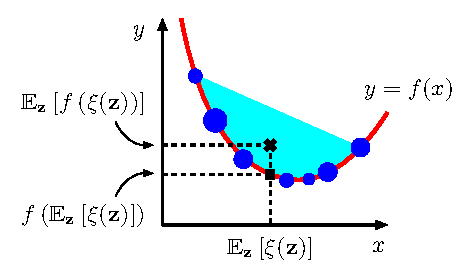
\includegraphics{jensen_inequality.eps}
\caption{A physical ``proof'' for
Jensen's inequality~\citep{MacKay:Information}.
Suppose that we have a set of point masses~$m_i = p(\mathbf{z}=\mathbf{z}_i)$,
denoted by filled blue circles ({\large\textcolor{blue}{$\bullet$}})
with areas proportional to $m_i$,
and place them at the corresponding
locations~$(x, y) = \left(\xi(\mathbf{z}_i), f(\xi(\mathbf{z}_i))\right)$
on a convex curve~$y = f(x)$.
The center of gravity of those masses, which is $\left(
\mathbb{E}_{\mathbf{z}}\left[\xi(\mathbf{z})\right],
\mathbb{E}_{\mathbf{z}}\left[f\left(\xi(\mathbf{z})\right)\right]
\right)$, denoted by a cross sign ($\boldsymbol{\times}$),
must lie above the convex curve and thus right above the point~$\left(
\mathbb{E}_{\mathbf{z}}\left[\xi(\mathbf{z})\right],
f\left(\mathbb{E}_{\mathbf{z}}\left[\xi(\mathbf{z})\right]\right)
\right)$ on the curve, denoted by a filled square ($\blacksquare$),
showing Jensen's inequality~\eqref{eq:Jensen_inequality_expectation_with_z}.
One can also see that, if $f(\cdot)$ is strictly convex,
the equality in \eqref{eq:Jensen_inequality_expectation_with_z}
implies that $\xi(\cdot)$ is constant (it is trivial to show that the converse is true). }
\label{fig:Jensen_inequality}
\end{figure}

\erratum{Page~80}
Equation~(2.52):
We usually take eigenvectors~$\mathbf{u}_{i}$ to be the columns of $\mathbf{U}$ as in (C.37).
If we follow this convention, (2.52) and the following text should read
\begin{equation}
\mathbf{y} = \mathbf{U}^{\operatorname{T}} (\mathbf{x} - \bm{\mu})
\label{eq:change_of_variable_x_to_y}
\end{equation}
where $\mathbf{U}$ is a matrix whose columns are given by $\mathbf{u}_{i}$ so that
$\mathbf{U} = \left( \mathbf{u}_{1}, \dots,  \mathbf{u}_{D}\right)$.
From (2.46) it follows that $\mathbf{U}$ is an \emph{orthogonal} matrix, i.e.,
it satisfies $\mathbf{U}^{\operatorname{T}}\mathbf{U} = \mathbf{I}$ and hence also
$\mathbf{U}\mathbf{U}^{\operatorname{T}} = \mathbf{I}$ where $\mathbf{I}$ is the identity matrix.

\erratum{Page~81}
Equations~(2.53) and (2.54):
If we write the change of variable from $\mathbf{x}$ to $\mathbf{y}$ as
\eqref{eq:change_of_variable_x_to_y} instead of (2.52),
the Jacobian matrix~$\mathbf{J} = \left( J_{ij} \right)$ is simply given by $\mathbf{U}$.
Equation~(2.53) should read
\begin{equation}
J_{ij} = \frac{\partial x_i}{\partial y_j} = U_{ij}
\end{equation}
where $U_{ij}$ is the $(ij)$-th element of $\mathbf{U}$.
The square of the determinant of the Jacobian matrix~(2.54) can then be evaluated as
\begin{equation}
\left| \mathbf{J} \right|^{2} = \left| \mathbf{U} \right|^{2}
= \left| \mathbf{U}^{\operatorname{T}} \right| \left| \mathbf{U} \right|
= \left| \mathbf{U}^{\operatorname{T}} \mathbf{U} \right|
= \left| \mathbf{I} \right| = 1.
\end{equation}

\erratum{Page~81}
Line~\textminus1:
Since the Jacobian matrix~$\mathbf{J}$ is only assumed to be orthogonal here,
the determinant of $\mathbf{J}$ can be either positive or negative so that
we should write $\left| \mathbf{J} \right| = \pm 1$
instead of $\left| \mathbf{J} \right| = 1$.

\erratum{Page~82}
Equation~(2.56):
We should take the absolute value of the determinant for the same reason given above;
the factor~$\left| \mathbf{J} \right|$ should read
$\left| \operatorname{det}\left( \mathbf{J} \right) \right|$.
Note that we cannot write $\left|\left| \mathbf{J} \right|\right|$ to mean
$\left| \operatorname{det}\left( \mathbf{J} \right) \right|$
because it is confusingly similar to the matrix norm~$\left\| \mathbf{J} \right\|$,
which usually refers to the largest singular value of $\mathbf{J}$~\citep{GvL:MC}.
This notational inconsistency has been caused by the abuse of the notation~$|\cdot|$ for
both the absolute value and the matrix determinant.
If we always use $\operatorname{det}(\cdot)$ for the determinant, confusion will not arise
and the notation be consistent.
An alternative solution to this problem would be to explicitly define
\begin{equation}
\left| \mathbf{A} \right| \equiv \left| \operatorname{det}\left( \mathbf{A} \right) \right|
\label{eq:abs_of_matrix_determinant}
\end{equation}
for any square matrix~$\mathbf{A}$ so that
we have $\left|\mathbf{J}\right| = 1$ and (2.56) holds as is.
Note also that this notation~\eqref{eq:abs_of_matrix_determinant} is mostly consistent
in other part of PRML because we have
$\left| \mathbf{A} \right| = \operatorname{det}\left( \mathbf{A} \right)$ for any positive
(semi)definite matrix~$\mathbf{A} \succeq 0$ (see Appendix~C) and
most matrices for which we take determinants, such as
the covariance~$\bm{\Sigma}$ or the precision~$\bm{\Lambda}$ of
the multivariate Gaussian distribution and
the scale matrix~$\mathbf{W}$ of the Wishart distribution,
are positive definite\footnote{In this report, we assume as customary that
the concept of positive/negative (semi)definiteness is restricted to symmetric matrices.
For example, when we say ``a matrix~$\mathbf{A}$ is positive definite'' or $\mathbf{A} \succ 0$,
$\mathbf{A}$ is also assumed to be symmetric so that $\mathbf{A}^{\operatorname{T}} = \mathbf{A}$,
though we still sometimes say ``$\mathbf{A}$ is symmetric positive definite'' to avoid confusion.
}.

\erratum{Pages~93 and 94}
Equations~(2.121) and (2.122):
We obtain the maximum likelihood solutions~$\bm{\mu}_\text{ML}$ and $\bm{\Sigma}_\text{ML}$
for the Gaussian by setting the derivatives of
the log likelihood function~$\ln p\left(\mathbf{X}\middle| \bm{\mu}, \bm{\Sigma}\right)$
given by (2.118) with respect to $\bm{\mu}$ and $\bm{\Sigma}$ equal to zero,
which, however, only implies that $\bm{\mu}_\text{ML}$ and $\bm{\Sigma}_\text{ML}$ are
stationary points.
We should also show that
$\bm{\mu}_\text{ML}$ and $\bm{\Sigma}_\text{ML}$ indeed maximize the likelihood.
This can be easily done for $\bm{\mu}_\text{ML}$ by noting that
the log likelihood~(2.118) is quadratic in $\bm{\mu}$ so that
\begin{equation}
\ln p\left(\mathbf{X}\middle| \bm{\mu}, \bm{\Sigma}\right) =
-\frac{N}{2}
\left(\bm{\mu} - \bm{\mu}_{\text{ML}}\right)^{\operatorname{T}} \bm{\Sigma}^{-1}
\left(\bm{\mu} - \bm{\mu}_{\text{ML}}\right)
+ \text{const}
\end{equation}
where $\bm{\mu}_{\text{ML}}$ is given by (2.121).
Since the covariance~$\bm{\Sigma}$ is positive definite and so is its inverse~$\bm{\Sigma}^{-1}$,
we see that the log likelihood is concave with respect to $\bm{\mu}$ and
that $\bm{\mu}_\text{ML}$ indeed maximizes the likelihood.
Next we consider $\bm{\Sigma}_\text{ML}$ given by (2.122), which we obtain by solving
\begin{equation}
\nabla_{\bm{\Sigma}} \ln p\left(\mathbf{X}\middle| \bm{\mu}_\text{ML}, \bm{\Sigma}\right)
= \mathbf{O}
\label{eq:maximum_likelihood_equation_for_covariance}
\end{equation}
where $\nabla_{\mathbf{A}}$ is the gradient operator with respect to a matrix~$\mathbf{A}$
defined by \eqref{eq:gradient_of_scalar_wrt_matrix} and
$\mathbf{O}$ is a zero matrix.
Making use of the eigenvalue expansion~(2.48) of $\bm{\Sigma}$,
we can write the log likelihood~(2.118) in terms of the eigenvalues~$\{\lambda_i\}$ so that
\begin{equation}
\ln p\left(\mathbf{X}\middle| \bm{\mu}, \bm{\Sigma}\right) =
-\frac{N}{2} \sum_{i=1}^{D} \left\{
\ln \lambda_i
+ \frac{S_i}{\lambda_i}
\right\}
+ \text{const}
\label{eq:log_likelihood_in_terms_of_eigenvalues}
\end{equation}
where
\begin{align}
S_{i} &= \frac{1}{N} \sum_{n=1}^{N} y_{ni}^{2} \\
y_{ni} &= \mathbf{u}_{i}^{\operatorname{T}}\left(\mathbf{x}_n - \bm{\mu}\right) .
\end{align}
From \eqref{eq:log_likelihood_in_terms_of_eigenvalues}, we see that
$\ln p\left(\mathbf{X}\middle| \bm{\mu}, \bm{\Sigma}\right) \to -\infty$
if $\bm{\Sigma}$ approaches the boundary of the space of symmetric positive definite matrices,
i.e., $\lambda_i \to 0$ or $\lambda_i \to \infty$.
Therefore, if \eqref{eq:maximum_likelihood_equation_for_covariance}
has a unique solution~$\bm{\Sigma}_\text{ML} \succ 0$,
then $\bm{\mu}_\text{ML}$ and $\bm{\Sigma}_\text{ML}$ jointly maximize the likelihood.
Note that a similar observation holds when we maximize the log likelihood in terms of
the precision~$\bm{\Lambda} \equiv \bm{\Sigma}^{-1}$
(in which case one can see that the log likelihood is concave also with respect to
the eigenvalues of $\bm{\Lambda}$).
See \citet{Anderson:MaximumLikelihood} for further discussions.

\erratum{Page~100}
Equations~(2.147) and (2.148):
We are also interested in the logarithmic expectation~$\mathbb{E}\left[ \ln\lambda \right]$
given by (B.30) because it is required to evaluate
the entropy~$\operatorname{H}\left[ \lambda \right]$ given by (B.31).
The logarithmic expectation~$\mathbb{E}\left[ \ln\lambda \right]$ can be easily calculated
by making use of the derivative of the gamma distribution~(2.146)
with respect to $a$, which is given by
\begin{equation}
\frac{\partial}{\partial a} \operatorname{Gam}\left(\lambda\middle|a, b\right)
= \left( \ln\lambda - \psi(a) + \ln b \right) \operatorname{Gam}\left(\lambda\middle|a, b\right)
\label{eq:derivative_of_gamma_distribution_wrt_a}
\end{equation}
where $\psi(\cdot)$ is the \emph{digamma} function defined by (B.25) so that
\begin{equation}
\psi(a) \equiv \frac{\mathrm{d}}{\mathrm{d}a} \ln \Gamma(a) = \frac{\Gamma'(a)}{\Gamma(a)} .
\end{equation}
Differentiating the both sides of the integral identity
\begin{equation}
\int_{0}^{\infty} \operatorname{Gam}\left(\lambda\middle|a, b\right) \mathrm{d}\lambda = 1
\end{equation}
with respect to $a$,
interchanging the order of the differentiation and the integral,
and substituting \eqref{eq:derivative_of_gamma_distribution_wrt_a},
we obtain
\begin{equation}
\mathbb{E}\left[ \ln \lambda \right] = \psi(a) - \ln b .
\end{equation}
It is worth noting here that the above expectation can also be written in the form
\begin{equation}
\mathbb{E}\left[ \ln \lambda \right] = \ln\frac{a}{b} - \varphi(a)
\end{equation}
where $\varphi(\cdot)$ is the \emph{log minus digamma} function defined by
\begin{equation}
\varphi(x) \equiv \ln x - \psi(x) .
\label{eq:log_minus_digamma_function}
\end{equation}
The log minus digamma function~$\varphi(\cdot)$ arises in
the maximum likelihood solutions for the gamma distribution~(2.146) as well as
in the EM algorithm for the Student's t-distribution~(2.159) or (2.162) in Exercise~12.24
as we shall see shortly.

\erratum{Page~102}
Equation~(2.155):
Although an interpretation for the parameters of the gamma distribution~(2.146) has been given,
no such an interpretation for the parameters of the Wishart distribution~(2.155) is given here
nor in Exercise~2.45.
Generally speaking, when we construct a probabilistic model with priors,
we must choose some reasonable initial values for their parameters, known as hyperparameters.
This calls for an intuitive interpretation for the parameters of such priors.
In order to give one for the parameters of the Wishart distribution,
let us consider a simple Bayesian inference problem in which,
given a set of $N$ observations~$\mathbf{X} =
\left\{ \mathbf{x}_1, \dots, \mathbf{x}_N \right\}$ for a zero-mean Gaussian random variable,
we infer the covariance matrix~$\bm{\Sigma}$ or, equivalently,
the precision matrix~$\bm{\Lambda} \equiv \bm{\Sigma}^{-1}$.
The likelihood~$p\left(\mathbf{X}\middle|\bm{\Lambda}\right)$
in terms of the precision~$\bm{\Lambda}$ is given by
\begin{equation}
p\left(\mathbf{X}\middle|\bm{\Lambda}\right) =
\prod_{n=1}^{N} p\left(\mathbf{x}_n\middle|\bm{\Lambda}\right) =
\prod_{n=1}^{N} \mathcal{N}\left(\mathbf{x}_n\middle|\mathbf{0}, \bm{\Lambda}^{-1}\right) .
\end{equation}
If we choose the prior~$p\left(\bm{\Lambda}\right)$ over $\bm{\Lambda}$ to be
a Wishart distribution so that
\begin{equation}
p\left(\bm{\Lambda}\right) = \mathcal{W}\left(\bm{\Lambda}\middle|\mathbf{W}_0, \nu_0\right)
\label{eq:wishart_prior}
\end{equation}
our analysis can be simplified because it is the conjugate prior.
In fact, the posterior~$p\left(\bm{\Lambda}\middle|\mathbf{X}\right)$ is given by
\begin{align}
p\left(\bm{\Lambda}\middle|\mathbf{X}\right) &\propto
p\left(\mathbf{X}\middle|\bm{\Lambda}\right) p\left(\bm{\Lambda}\right) \\
&\propto \left|\bm{\Lambda}\right|^{N/2}
\exp\left\{-\frac{1}{2}\sum_{n=1}^{N}\mathbf{x}_n^{\operatorname{T}}\bm{\Lambda}\mathbf{x}_n\right\}
\left|\bm{\Lambda}\right|^{(\nu_0 - D - 1)/2}
\exp\left\{-\frac{1}{2}\operatorname{Tr}\left(\mathbf{W}_0^{-1}\bm{\Lambda}\right)\right\} \\
&= \left|\bm{\Lambda}\right|^{(\nu_N - D - 1)/2}
\exp\left\{-\frac{1}{2}\operatorname{Tr}\left(\mathbf{W}_N^{-1}\bm{\Lambda}\right)\right\}
\end{align}
where
\begin{align}
\nu_N &= \nu_0 + N \\
\mathbf{W}_N^{-1} &=
\mathbf{W}_0^{-1} + \sum_{n=1}^{N}\mathbf{x}_n\mathbf{x}_n^{\operatorname{T}} .
\end{align}
Reinstating the normalization constant, we indeed see that the posterior becomes again
a Wishart distribution of the form
\begin{equation}
p\left(\bm{\Lambda}\middle|\mathbf{X}\right) =
\mathcal{W}\left(\bm{\Lambda}\middle|\mathbf{W}_N, \nu_N\right) .
\end{equation}
This result suggests us how we can interpret the parameters of
the Wishart distribution~(2.155), namely
the scale matrix~$\mathbf{W}$ and the number of degrees of freedom~$\nu$.
Since observing $N$ data points increases the number of degrees of freedom~$\nu$ by $N$,
we can interpret $\nu_0$ in the prior~\eqref{eq:wishart_prior} as
the number of ``effective'' prior observations.
The $N$ observations also contribute $N\bm{\Sigma}_{\text{ML}}$ to
the inverse of the scale matrix~$\mathbf{W}$
where $\bm{\Sigma}_{\text{ML}}$ is the maximum likelihood estimate for the covariance of
the observations given by
\begin{equation}
\bm{\Sigma}_{\text{ML}} = \frac{1}{N} \sum_{n=1}^{N}\mathbf{x}_n\mathbf{x}_n^{\operatorname{T}} .
\end{equation}
This suggests an interpretation of $\mathbf{W}$ in terms of the ``covariance'' parameter
\begin{equation}
\bm{\Sigma} \equiv \left(\nu\mathbf{W}\right)^{-1} .
\label{eq:covariance_parameter}
\end{equation}
More specifically, we can interpret $\bm{\Sigma}_0 = \left(\nu_0\mathbf{W}_0\right)^{-1}$ as
the covariance of the $\nu_0$ ``effective'' prior observations.
Note that this interpretation is in accordance with another observation that
the expectation of $\bm{\Lambda}$ with respect to
the prior~\eqref{eq:wishart_prior} is indeed given by
$\mathbb{E}\left[\bm{\Lambda}\right] = \nu_0\mathbf{W}_0 = \bm{\Sigma}_0^{-1}$
where we have used (B.80).

\erratum{Page~102}
Equation~(2.157):
Again, no interpretation is given for the parameters of the Gaussian-Wishart distribution~(2.157)
nor for those of the Gaussian-gamma distribution~(2.154).
Since the Gaussian-gamma can be obtained as a special case of the Gaussian-Wishart
where the dimension is one so that $D=1$,
we shall make an interpretation only for the parameters of the Gaussian-Wishart here.
Let us consider a problem of inferring the mean~$\bm{\mu}$ and the precision~$\bm{\Lambda}$ given
the Gaussian likelihood
\begin{equation}
p\left(\mathbf{X}\middle|\bm{\mu}, \bm{\Lambda}\right) =
\prod_{n=1}^{N} \mathcal{N}\left(\mathbf{x}_n\middle|\bm{\mu}, \bm{\Lambda}^{-1}\right)
\end{equation}
and the Gaussian-Wishart prior
\begin{equation}
p\left(\bm{\mu}, \bm{\Lambda}\right) =
\mathcal{N}\left(\bm{\mu}\middle|\bm{\mu}_0, \left(\beta_0\bm{\Lambda}\right)^{-1}\right)
\mathcal{W}\left(\bm{\Lambda}\middle|\mathbf{W}_0, \nu_0\right) .
\end{equation}
At this moment, we introduce notations for the maximum likelihood estimates for
the mean and the covariance
given the $N$ observations~$\mathbf{X} = \left\{ \mathbf{x}_1, \dots, \mathbf{x}_N \right\}$,
i.e.,
\begin{equation}
\bm{\mu}_{\text{ML}} = \frac{1}{N} \sum_{n=1}^{N} \mathbf{x}_n, \qquad
\bm{\Sigma}_{\text{ML}} =
\frac{1}{N} \sum_{n=1}^{N}
(\mathbf{x}_n - \bm{\mu}_{\text{ML}})
(\mathbf{x}_n - \bm{\mu}_{\text{ML}})^{\operatorname{T}}
\end{equation}
respectively.
Evaluating the posterior, we have
\begin{align}
p\left(\bm{\mu}, \bm{\Lambda}\middle|\mathbf{X}\right) &\propto
p\left(\mathbf{X}\middle|\bm{\mu}, \bm{\Lambda}\right)
p\left(\bm{\mu}, \bm{\Lambda}\right) \\
&\propto
\left|\bm{\Lambda}\right|^{N/2}
\exp\left\{-\frac{1}{2}\sum_{n=1}^{N}
  \left(\mathbf{x}_n - \bm{\mu}\right)^{\operatorname{T}} \bm{\Lambda}
  \left(\mathbf{x}_n - \bm{\mu}\right)
\right\} \nonumber \\
&\phantom{\propto} \times
\left|\bm{\Lambda}\right|^{(\nu_0 - D)/2}
\exp\left\{-\frac{1}{2}\operatorname{Tr}\left(\left\{
\mathbf{W}_{0}^{-1} +
\beta_0\left(\bm{\mu} - \bm{\mu}_0\right)\left(\bm{\mu} - \bm{\mu}_0\right)^{\operatorname{T}}
\right\}\bm{\Lambda}\right)\right\} \\
&=
\left|\bm{\Lambda}\right|^{(\nu_N - D)/2}
\exp\left\{-\frac{1}{2}\operatorname{Tr}\left(\left\{
\mathbf{W}_{N}^{-1} +
\beta_N\left(\bm{\mu} - \bm{\mu}_N\right)\left(\bm{\mu} - \bm{\mu}_N\right)^{\operatorname{T}}
\right\}\bm{\Lambda}\right)\right\}
\end{align}
where
\begin{align}
\beta_N &= \beta_0 + N \\
\beta_N\bm{\mu}_N &= \beta_0\bm{\mu}_0 + N\bm{\mu}_{\text{ML}} \\
\nu_N &= \nu_0 + N \\
\mathbf{W}_{N}^{-1} &= \mathbf{W}_{0}^{-1} + N \bm{\Sigma}_{\text{ML}} +
\frac{\beta_0 N}{\beta_0 + N}
\left(\bm{\mu}_{\text{ML}} - \bm{\mu}_0\right)
\left(\bm{\mu}_{\text{ML}} - \bm{\mu}_0\right)^{\operatorname{T}} .
\label{eq:Gaussian-Wishart_W_0}
\end{align}
Thus, we find that the posterior is again a Gaussian-Wishart of the form
\begin{equation}
p\left(\bm{\mu}, \bm{\Lambda}\middle|\mathbf{X}\right) =
\mathcal{N}\left(\bm{\mu}\middle|\bm{\mu}_N, \left(\beta_N\bm{\Lambda}\right)^{-1}\right)
\mathcal{W}\left(\bm{\Lambda}\middle|\mathbf{W}_N, \nu_N\right) .
\end{equation}
From this result, we see that
the parameters~$\beta_0$ and $\bm{\mu}_0$ for the mean~$\bm{\mu}$ are basically
(but not completely) separate from
the parameters~$\nu_0$ and $\mathbf{W}_0$ for the precision~$\bm{\Lambda}$.
We can interpret $\beta_0$ as the number of ``effective'' prior observations for the mean and
$\bm{\mu}_0$ as the mean of the $\beta_0$ prior observations.
The interpretation of $\nu_0$ and $\mathbf{W}_0$ is similar to
the one we have made in the previous erratum except that
we have in \eqref{eq:Gaussian-Wishart_W_0} a term due to the uncertainty in the mean,
that is, the difference between the maximum likelihood mean~$\bm{\mu}_{\text{ML}}$ and
the prior mean~$\bm{\mu}_0$.
Note that a similar result is obtained in Section~10.2.1 for a Bayesian mixture of Gaussians model
in which we assume a Gaussian-Wishart prior for each Gaussian component.

\erratum{Page~102}
Line~\textminus2:
``Gamma'' should read ``gamma'' (without capitalization).

\erratum{Page~103}
Figure~2.15: The tails of the Student's t-distributions are too high;
one can easily see that, if compared to the corresponding Gaussian distribution
labeled $\nu\to\infty$,
the t-distributions are not correctly normalized.
Figure~\ref{fig:Student_t_densities} gives the correct plot.

\begin{figure}
\centering
% GNUPLOT: LaTeX picture with Postscript
\begingroup
  \makeatletter
  \providecommand\color[2][]{%
    \GenericError{(gnuplot) \space\space\space\@spaces}{%
      Package color not loaded in conjunction with
      terminal option `colourtext'%
    }{See the gnuplot documentation for explanation.%
    }{Either use 'blacktext' in gnuplot or load the package
      color.sty in LaTeX.}%
    \renewcommand\color[2][]{}%
  }%
  \providecommand\includegraphics[2][]{%
    \GenericError{(gnuplot) \space\space\space\@spaces}{%
      Package graphicx or graphics not loaded%
    }{See the gnuplot documentation for explanation.%
    }{The gnuplot epslatex terminal needs graphicx.sty or graphics.sty.}%
    \renewcommand\includegraphics[2][]{}%
  }%
  \providecommand\rotatebox[2]{#2}%
  \@ifundefined{ifGPcolor}{%
    \newif\ifGPcolor
    \GPcolortrue
  }{}%
  \@ifundefined{ifGPblacktext}{%
    \newif\ifGPblacktext
    \GPblacktextfalse
  }{}%
  % define a \g@addto@macro without @ in the name:
  \let\gplgaddtomacro\g@addto@macro
  % define empty templates for all commands taking text:
  \gdef\gplbacktext{}%
  \gdef\gplfronttext{}%
  \makeatother
  \ifGPblacktext
    % no textcolor at all
    \def\colorrgb#1{}%
    \def\colorgray#1{}%
  \else
    % gray or color?
    \ifGPcolor
      \def\colorrgb#1{\color[rgb]{#1}}%
      \def\colorgray#1{\color[gray]{#1}}%
      \expandafter\def\csname LTw\endcsname{\color{white}}%
      \expandafter\def\csname LTb\endcsname{\color{black}}%
      \expandafter\def\csname LTa\endcsname{\color{black}}%
      \expandafter\def\csname LT0\endcsname{\color[rgb]{1,0,0}}%
      \expandafter\def\csname LT1\endcsname{\color[rgb]{0,1,0}}%
      \expandafter\def\csname LT2\endcsname{\color[rgb]{0,0,1}}%
      \expandafter\def\csname LT3\endcsname{\color[rgb]{1,0,1}}%
      \expandafter\def\csname LT4\endcsname{\color[rgb]{0,1,1}}%
      \expandafter\def\csname LT5\endcsname{\color[rgb]{1,1,0}}%
      \expandafter\def\csname LT6\endcsname{\color[rgb]{0,0,0}}%
      \expandafter\def\csname LT7\endcsname{\color[rgb]{1,0.3,0}}%
      \expandafter\def\csname LT8\endcsname{\color[rgb]{0.5,0.5,0.5}}%
    \else
      % gray
      \def\colorrgb#1{\color{black}}%
      \def\colorgray#1{\color[gray]{#1}}%
      \expandafter\def\csname LTw\endcsname{\color{white}}%
      \expandafter\def\csname LTb\endcsname{\color{black}}%
      \expandafter\def\csname LTa\endcsname{\color{black}}%
      \expandafter\def\csname LT0\endcsname{\color{black}}%
      \expandafter\def\csname LT1\endcsname{\color{black}}%
      \expandafter\def\csname LT2\endcsname{\color{black}}%
      \expandafter\def\csname LT3\endcsname{\color{black}}%
      \expandafter\def\csname LT4\endcsname{\color{black}}%
      \expandafter\def\csname LT5\endcsname{\color{black}}%
      \expandafter\def\csname LT6\endcsname{\color{black}}%
      \expandafter\def\csname LT7\endcsname{\color{black}}%
      \expandafter\def\csname LT8\endcsname{\color{black}}%
    \fi
  \fi
    \setlength{\unitlength}{0.0500bp}%
    \ifx\gptboxheight\undefined%
      \newlength{\gptboxheight}%
      \newlength{\gptboxwidth}%
      \newsavebox{\gptboxtext}%
    \fi%
    \setlength{\fboxrule}{0.5pt}%
    \setlength{\fboxsep}{1pt}%
\begin{picture}(4680.00,3024.00)%
    \gplgaddtomacro\gplbacktext{%
      \csname LTb\endcsname%
      \put(459,372){\makebox(0,0)[r]{\strut{}$0$}}%
      \csname LTb\endcsname%
      \put(459,962){\makebox(0,0)[r]{\strut{}$0.1$}}%
      \csname LTb\endcsname%
      \put(459,1551){\makebox(0,0)[r]{\strut{}$0.2$}}%
      \csname LTb\endcsname%
      \put(459,2141){\makebox(0,0)[r]{\strut{}$0.3$}}%
      \csname LTb\endcsname%
      \put(459,2731){\makebox(0,0)[r]{\strut{}$0.4$}}%
      \csname LTb\endcsname%
      \put(561,186){\makebox(0,0){\strut{}$-5$}}%
      \csname LTb\endcsname%
      \put(933,186){\makebox(0,0){\strut{}$-4$}}%
      \csname LTb\endcsname%
      \put(1677,186){\makebox(0,0){\strut{}$-2$}}%
      \csname LTb\endcsname%
      \put(2421,186){\makebox(0,0){\strut{}$0$}}%
      \csname LTb\endcsname%
      \put(3164,186){\makebox(0,0){\strut{}$2$}}%
      \csname LTb\endcsname%
      \put(3908,186){\makebox(0,0){\strut{}$4$}}%
      \csname LTb\endcsname%
      \put(4280,186){\makebox(0,0){\strut{}$5$}}%
    }%
    \gplgaddtomacro\gplfronttext{%
      \csname LTb\endcsname%
      \put(144,1595){\rotatebox{-270}{\makebox(0,0){\strut{}}}}%
      \csname LTb\endcsname%
      \put(4465,1595){\rotatebox{-270}{\makebox(0,0){\strut{}}}}%
      \csname LTb\endcsname%
      \put(2420,2726){\makebox(0,0){\strut{}}}%
      \csname LTb\endcsname%
      \put(2420,2725){\makebox(0,0){\strut{}}}%
      \csname LTb\endcsname%
      \put(51,93){\makebox(0,0)[l]{\strut{}}}%
      \csname LTb\endcsname%
      \put(3668,2634){\makebox(0,0){\strut{}}}%
      \colorrgb{0.00,1.00,0.00}%
      \put(3362,2522){\makebox(0,0)[l]{\strut{}$\nu \to \infty$}}%
      \colorrgb{0.00,0.00,1.00}%
      \put(3362,2299){\makebox(0,0)[l]{\strut{}$\nu = 1$}}%
      \colorrgb{1.00,0.00,0.00}%
      \put(3362,2076){\makebox(0,0)[l]{\strut{}$\nu = 0.1$}}%
    }%
    \gplbacktext
    \put(0,0){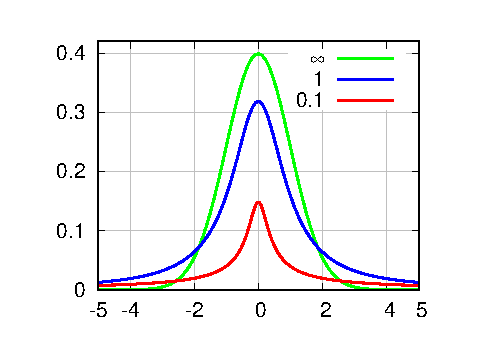
\includegraphics{student_t_plots}}%
    \gplfronttext
  \end{picture}%
\endgroup
~%
% GNUPLOT: LaTeX picture with Postscript
\begingroup
  \makeatletter
  \providecommand\color[2][]{%
    \GenericError{(gnuplot) \space\space\space\@spaces}{%
      Package color not loaded in conjunction with
      terminal option `colourtext'%
    }{See the gnuplot documentation for explanation.%
    }{Either use 'blacktext' in gnuplot or load the package
      color.sty in LaTeX.}%
    \renewcommand\color[2][]{}%
  }%
  \providecommand\includegraphics[2][]{%
    \GenericError{(gnuplot) \space\space\space\@spaces}{%
      Package graphicx or graphics not loaded%
    }{See the gnuplot documentation for explanation.%
    }{The gnuplot epslatex terminal needs graphicx.sty or graphics.sty.}%
    \renewcommand\includegraphics[2][]{}%
  }%
  \providecommand\rotatebox[2]{#2}%
  \@ifundefined{ifGPcolor}{%
    \newif\ifGPcolor
    \GPcolortrue
  }{}%
  \@ifundefined{ifGPblacktext}{%
    \newif\ifGPblacktext
    \GPblacktextfalse
  }{}%
  % define a \g@addto@macro without @ in the name:
  \let\gplgaddtomacro\g@addto@macro
  % define empty templates for all commands taking text:
  \gdef\gplbacktext{}%
  \gdef\gplfronttext{}%
  \makeatother
  \ifGPblacktext
    % no textcolor at all
    \def\colorrgb#1{}%
    \def\colorgray#1{}%
  \else
    % gray or color?
    \ifGPcolor
      \def\colorrgb#1{\color[rgb]{#1}}%
      \def\colorgray#1{\color[gray]{#1}}%
      \expandafter\def\csname LTw\endcsname{\color{white}}%
      \expandafter\def\csname LTb\endcsname{\color{black}}%
      \expandafter\def\csname LTa\endcsname{\color{black}}%
      \expandafter\def\csname LT0\endcsname{\color[rgb]{1,0,0}}%
      \expandafter\def\csname LT1\endcsname{\color[rgb]{0,1,0}}%
      \expandafter\def\csname LT2\endcsname{\color[rgb]{0,0,1}}%
      \expandafter\def\csname LT3\endcsname{\color[rgb]{1,0,1}}%
      \expandafter\def\csname LT4\endcsname{\color[rgb]{0,1,1}}%
      \expandafter\def\csname LT5\endcsname{\color[rgb]{1,1,0}}%
      \expandafter\def\csname LT6\endcsname{\color[rgb]{0,0,0}}%
      \expandafter\def\csname LT7\endcsname{\color[rgb]{1,0.3,0}}%
      \expandafter\def\csname LT8\endcsname{\color[rgb]{0.5,0.5,0.5}}%
    \else
      % gray
      \def\colorrgb#1{\color{black}}%
      \def\colorgray#1{\color[gray]{#1}}%
      \expandafter\def\csname LTw\endcsname{\color{white}}%
      \expandafter\def\csname LTb\endcsname{\color{black}}%
      \expandafter\def\csname LTa\endcsname{\color{black}}%
      \expandafter\def\csname LT0\endcsname{\color{black}}%
      \expandafter\def\csname LT1\endcsname{\color{black}}%
      \expandafter\def\csname LT2\endcsname{\color{black}}%
      \expandafter\def\csname LT3\endcsname{\color{black}}%
      \expandafter\def\csname LT4\endcsname{\color{black}}%
      \expandafter\def\csname LT5\endcsname{\color{black}}%
      \expandafter\def\csname LT6\endcsname{\color{black}}%
      \expandafter\def\csname LT7\endcsname{\color{black}}%
      \expandafter\def\csname LT8\endcsname{\color{black}}%
    \fi
  \fi
    \setlength{\unitlength}{0.0500bp}%
    \ifx\gptboxheight\undefined%
      \newlength{\gptboxheight}%
      \newlength{\gptboxwidth}%
      \newsavebox{\gptboxtext}%
    \fi%
    \setlength{\fboxrule}{0.5pt}%
    \setlength{\fboxsep}{1pt}%
\begin{picture}(4680.00,3024.00)%
    \gplgaddtomacro\gplbacktext{%
      \csname LTb\endcsname%
      \put(459,372){\makebox(0,0)[r]{\strut{}$-10$}}%
      \csname LTb\endcsname%
      \put(459,861){\makebox(0,0)[r]{\strut{}$-8$}}%
      \csname LTb\endcsname%
      \put(459,1351){\makebox(0,0)[r]{\strut{}$-6$}}%
      \csname LTb\endcsname%
      \put(459,1840){\makebox(0,0)[r]{\strut{}$-4$}}%
      \csname LTb\endcsname%
      \put(459,2330){\makebox(0,0)[r]{\strut{}$-2$}}%
      \csname LTb\endcsname%
      \put(459,2819){\makebox(0,0)[r]{\strut{}$0$}}%
      \csname LTb\endcsname%
      \put(561,186){\makebox(0,0){\strut{}$-15$}}%
      \csname LTb\endcsname%
      \put(1181,186){\makebox(0,0){\strut{}$-10$}}%
      \csname LTb\endcsname%
      \put(1801,186){\makebox(0,0){\strut{}$-5$}}%
      \csname LTb\endcsname%
      \put(2421,186){\makebox(0,0){\strut{}$0$}}%
      \csname LTb\endcsname%
      \put(3040,186){\makebox(0,0){\strut{}$5$}}%
      \csname LTb\endcsname%
      \put(3660,186){\makebox(0,0){\strut{}$10$}}%
      \csname LTb\endcsname%
      \put(4280,186){\makebox(0,0){\strut{}$15$}}%
    }%
    \gplgaddtomacro\gplfronttext{%
      \csname LTb\endcsname%
      \put(144,1595){\rotatebox{-270}{\makebox(0,0){\strut{}}}}%
      \csname LTb\endcsname%
      \put(4465,1595){\rotatebox{-270}{\makebox(0,0){\strut{}}}}%
      \csname LTb\endcsname%
      \put(2420,2726){\makebox(0,0){\strut{}}}%
      \csname LTb\endcsname%
      \put(2420,2725){\makebox(0,0){\strut{}}}%
      \csname LTb\endcsname%
      \put(51,93){\makebox(0,0)[l]{\strut{}}}%
      \csname LTb\endcsname%
      \put(3668,2634){\makebox(0,0){\strut{}}}%
      \colorrgb{0.00,1.00,0.00}%
      \put(3362,2522){\makebox(0,0)[l]{\strut{}$\nu \to \infty$}}%
      \colorrgb{0.00,0.00,1.00}%
      \put(3362,2299){\makebox(0,0)[l]{\strut{}$\nu = 1$}}%
      \colorrgb{1.00,0.00,0.00}%
      \put(3362,2076){\makebox(0,0)[l]{\strut{}$\nu = 0.1$}}%
    }%
    \gplbacktext
    \put(0,0){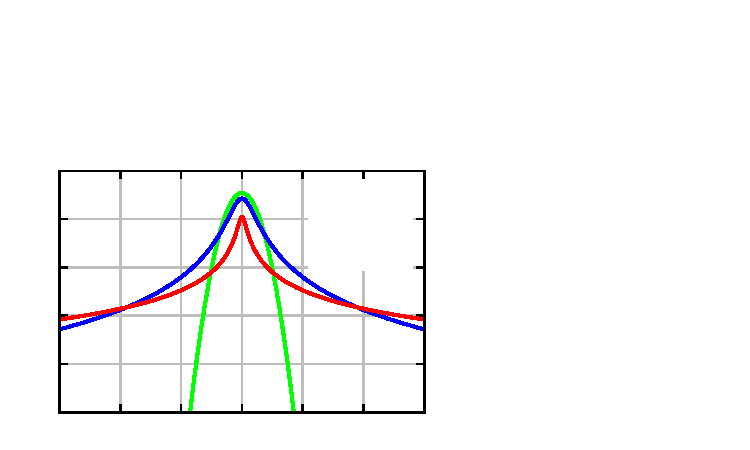
\includegraphics{student_t_plots_log}}%
    \gplfronttext
  \end{picture}%
\endgroup

\caption{Plot of Student's t-distribution density
functions~$\operatorname{St}\left(x\middle|\mu, \lambda, \nu\right)$ (left) and
corresponding log density
functions~$\ln\operatorname{St}\left(x\middle|\mu, \lambda, \nu\right)$ (right)
for various values of $\nu$ where we have fixed $\mu = 0$ and $\lambda = 1$. }
\label{fig:Student_t_densities}
\end{figure}

\erratum{Page~104}
The text after (2.160):
The Gaussian~$\mathcal{N}\left(\mathbf{x}\middle|\bm{\mu}, \mathbf{\Lambda}\right)$
should read $\mathcal{N}\left(\mathbf{x}\middle|\bm{\mu}, \mathbf{\Lambda}^{-1}\right)$.

\erratum{Page~116}
Equation~(2.224):
The right hand side should be a zero vector~$\mathbf{0}$.

\erratum{Page~126}
% See http://ibisforest.org/index.php?PRML%2Ferrata1
Figure~2.28: 
The red, green, and blue points correspond to
the ``homogeneous,'' ``annular,'' and ``laminar (or stratified)'' classes, respectively.

\erratum{Page~129}
Exercise~2.9:
Remove the period (.) after \www.

\erratum{Page~141}
Equation~(3.13):
The use of the gradient operator~$\nabla$ is not consistent here.
As in (2.224), the gradient of a scalar function is usually defined as a column vector
of derivatives so that (3.13) should read\footnote{\
Note that we use a different typeface for
the data vector~$\bm{\mathsf{t}} = \left( t_1, \dots, t_N \right)^{\operatorname{T}}$.
See ``Mathematical notation'' on page xi of PRML.}
\begin{equation}
\nabla \ln p \left( \bm{\mathsf{t}} \middle| \mathbf{w}, \beta \right) =
\beta \sum_{n=1}^{N}
\left\{ t_n - \mathbf{w}^{\operatorname{T}} \bm{\phi}\left( \mathbf{x}_n \right) \right\}
\bm{\phi}\left( \mathbf{x}_n \right) .
\label{eq:gradient_of_linear_regression_likelihood}
\end{equation}
Moreover, I would like to also suggest that we should give a definition for the gradient
before we use it or, at least, in an appendix.
Although Appendix~C defines the vector derivative~$\frac{\partial}{\partial \mathbf{x}}$,
which is used interchangeably with the gradient~$\nabla_{\mathbf{x}}$ throughout PRML,
there is no mention of the gradient.
We shall come back to this issue later in this report.

\erratum{Page~142}
Equation~(3.14):
The left hand side should be a zero vector~$\mathbf{0}$ instead of a scalar zero~$0$.
Thus, (3.14) should read
\begin{equation}
\mathbf{0} =
\sum_{n=1}^{N} t_n \bm{\phi}\left( \mathbf{x}_n \right)
- \left( \sum_{n=1}^{N}
\bm{\phi}\left(\mathbf{x}_n\right)\bm{\phi}\left(\mathbf{x}_n\right)^{\operatorname{T}} \right)
\mathbf{w}
\end{equation}
where we have used the gradient of the form~\eqref{eq:gradient_of_linear_regression_likelihood}
instead of (3.13).

\erratum{Page~146}
Equation~(3.31):
The left hand side should be $\mathbf{y}\left(\mathbf{x}, \mathbf{W}\right)$ instead of
$\mathbf{y}\left(\mathbf{x}, \mathbf{w}\right)$.

\erratum{Page~166}
The second paragraph, Line~1:
``Gamma'' should read ``gamma'' (without capitalization).

\erratum{Pages~168--169, and 177}
Equations~(3.88), (3.93), and (3.117) as well as the text before (3.93):
The derivative operators should be partial differentials.
For example, (3.117) should read
\begin{equation}
\frac{\partial}{\partial \alpha} \ln \left| \mathbf{A} \right| =
\operatorname{Tr}\left( \mathbf{A}^{-1} \frac{\partial}{\partial \alpha} \mathbf{A} \right) .
\end{equation}

\erratum{Page~170}
Figure~3.15:
The eigenvectors~$\mathbf{u}_{i}$ are unit vectors.
The scaled vectors~$\mathbf{u}_{1}$ and $\mathbf{u}_{2}$ in Figure~3.15 should be labeled as
$\lambda_{1}^{-1/2}\mathbf{u}_{1}$ and $\lambda_{2}^{-1/2}\mathbf{u}_{2}$.

\erratum{Page~179}
Line~9:
The decision surfaces are defined by linear \emph{equations} of the input vector~$\mathbf{x}$ and
thus are $(D - 1)$-dimensional hyperplanes within the $D$-dimensional input space.

\erratum{Page~207}
Equation~(4.92):
The gradient and the Hessian in the right hand side,
which are in general functions of the parameter~$\mathbf{w}$,
must be evaluated at the previous estimate~$\mathbf{w}^{\text{old}}$ for the parameter.
Thus, (4.92) should read
\begin{equation}
\mathbf{w}^{\text{new}} = \mathbf{w}^{\text{old}} -
  \left[ \mathbf{H} \left( \mathbf{w}^{\text{old}} \right) \right]^{-1}
  \nabla E \left( \mathbf{w}^{\text{old}} \right)
\end{equation}
where $\mathbf{H}\left(\mathbf{w}\right) \equiv \nabla\nabla E\left(\mathbf{w}\right)$ is
the Hessian matrix whose elements comprise the second derivatives of $E\left(\mathbf{w}\right)$
with respect to the components of $\mathbf{w}$.

\erratum{Page~210}
Equation~(4.110) and the preceding text:
The left hand side of (4.110) is obtained by taking the gradient of $\nabla_{\mathbf{w}_{j}} E$
given in (4.109) with respect to $\mathbf{w}_{k}$ and corresponds to
the $(k, j)$-th block of the Hessian, \emph{not} the $(j, k)$-th.
Thus, (4.110) should read
\begin{equation}
\nabla_{\mathbf{w}_{k}} \nabla_{\mathbf{w}_{j}}
E \left( \mathbf{w}_{1}, \dots, \mathbf{w}_{K} \right)
  = \sum_{n=1}^{N} y_{nj} \left( I_{kj} - y_{nk} \right)
    \bm{\phi}_{n} \bm{\phi}_{n}^{\operatorname{T}}.
\end{equation}
To be clear, we have used the following notation.
If we group all the parameters~$\mathbf{w}_{1}$, $\dots$, $\mathbf{w}_{K}$ into
a column vector
\begin{equation}
\mathbf{w} =
  \begin{pmatrix}
  \mathbf{w}_{1} \\
  \vdots \\
  \mathbf{w}_{K}
  \end{pmatrix}
\end{equation}
the gradient and the Hessian of the error function~$E\left(\mathbf{w}\right)$ with respect to
$\mathbf{w}$ are given by
\begin{equation}
\nabla_{\mathbf{w}} E =
  \begin{pmatrix}
  \nabla_{\mathbf{w}_{1}} E \\
  \vdots \\
  \nabla_{\mathbf{w}_{K}} E
  \end{pmatrix} , \qquad
\nabla_{\mathbf{w}} \nabla_{\mathbf{w}} E =
  \begin{pmatrix}
  \nabla_{\mathbf{w}_{1}} \nabla_{\mathbf{w}_{1}} E &
  \cdots &
  \nabla_{\mathbf{w}_{1}} \nabla_{\mathbf{w}_{K}} E \\
  \vdots & \ddots & \vdots \\
  \nabla_{\mathbf{w}_{K}} \nabla_{\mathbf{w}_{1}} E &
  \cdots &
  \nabla_{\mathbf{w}_{K}} \nabla_{\mathbf{w}_{K}} E
  \end{pmatrix}
\end{equation}
respectively.

\erratum{Page~239}
Figure~5.6:
The eigenvectors~$\mathbf{u}_{1}$ and $\mathbf{u}_{2}$ should be unit vectors.
Thus, their orientations should be shown as in Figure~2.7.
Or, the scaled vectors should be labeled as
$\lambda_{1}^{-1/2}\mathbf{u}_{1}$ and $\lambda_{2}^{-1/2}\mathbf{u}_{2}$.

\erratum{Page~251}
The second paragraph:
The outer product approximation to the Hessian of the form~(5.84) is usually referred to as
the \emph{Gauss-Newton} approximation~\citep{Press:NR},
which not only eliminates the computation of second derivatives
but also guarantees that the Hessian thus approximated is positive (semi)definite,
whereas the \emph{Levenberg-Marquardt} method~\citep{Press:NR} is a method that improves
the numerical stability of (Gauss\nobreakdash-)Newton type iterations
by correcting the Hessian matrix so as to be more diagonal dominant.
Let us now compare the two types of approximation to the Hessian, i.e.,
Gauss-Newton and Levenberg-Marquardt, more specifically in the following.
We first observe that the Gauss-Newton approximation to the Hessian
given in the right hand side of (5.84)
can be written succinctly in terms of matrix product as
\begin{equation}
\mathbf{H}_{\text{GN}} = \mathbf{J}^{\operatorname{T}}\mathbf{J}
\end{equation}
where $\mathbf{J} = \left( \nabla a_1, \dots, \nabla a_N \right)^{\operatorname{T}}$ is
the Jacobian of the activations~$a_1, \dots, a_N$ with respect to the parameters
(weights and biases).
The Levenberg-Marquardt approximation to the above Hessian typically takes the form
\begin{equation}
\mathbf{H}_{\text{LM}} = \mathbf{J}^{\operatorname{T}}\mathbf{J} + \lambda \mathbf{I}
\end{equation}
or
\begin{equation}
\mathbf{H}_{\text{LM}} = \mathbf{J}^{\operatorname{T}}\mathbf{J}
+ \lambda \operatorname{diag}\left( \mathbf{J}^{\operatorname{T}}\mathbf{J} \right)
\end{equation}
where we have introduced an adjustable damping factor~$\lambda \geqslant 0$
(which will be adjusted through the iterations) and defined that,
for a square matrix~$\mathbf{A} = (A_{ij})$, $\operatorname{diag}(\mathbf{A})$ is
a diagonal matrix obtained by setting the non-diagonal elements equal to zero so that
$\operatorname{diag}(\mathbf{A}) = \operatorname{diag}(A_{ii})$.

\erratum{Page~259}
% See http://ibisforest.org/index.php?PRML%2Ferrata1
Line~2:
The parameters rescaling should be
$\lambda_1 \to a^2\lambda_1$ and $\lambda_2 \to c^{-2}\lambda_2$.

\erratum{Page~275}
The text after (5.154):
The identity matrix~$\mathbf{I}$ should multiply $\sigma_{k}^{2}(\mathbf{x}_{n})$.

\erratum{Page~277}
Equation~(5.160):
The factor~$L$ should multiply $\sigma_{k}^{2}(\mathbf{x})$ because we have
\begin{align}
s^2(\mathbf{x}) &=
  \mathbb{E}\left[
    \operatorname{Tr}\left\{
      \left( \mathbf{t} - \mathbb{E}\left[ \mathbf{t} \middle| \mathbf{x} \right] \right)
      \left( \mathbf{t} - \mathbb{E}\left[ \mathbf{t} \middle| \mathbf{x} \right]
        \right)^{\operatorname{T}} \right\}
  \middle| \mathbf{x} \right] \\
&= \sum_{k=1}^{K} \pi_{k}(\mathbf{x})
  \operatorname{Tr}\left\{ \sigma_{k}^{2}(\mathbf{x})\mathbf{I} +
    \left( \bm{\mu}_{k}(\mathbf{x}) -
      \mathbb{E}\left[ \mathbf{t} \middle| \mathbf{x} \right] \right)
    \left( \bm{\mu}_{k}(\mathbf{x}) -
      \mathbb{E}\left[ \mathbf{t} \middle| \mathbf{x} \right] \right)^{\operatorname{T}}
  \right\} \\
&= \sum_{k=1}^{K} \pi_{k}(\mathbf{x})
  \left\{ L \sigma_{k}^{2}(\mathbf{x}) +
    \left\| \bm{\mu}_{k}(\mathbf{x}) -
      \mathbb{E}\left[ \mathbf{t} \middle| \mathbf{x} \right] \right\|^{2}
  \right\}
\end{align}
where $L$ is the dimensionality of $\mathbf{t}$.

\erratum{Page~295}
Line~1:
The vector~$\mathbf{x}$ should be a column vector so that
$\mathbf{x} = \left( x_1, x_2 \right)^{\operatorname{T}}$.

\erratum{Page~318}
Equations~(6.93) and (6.94)
as well as the text before (6.93):
The text and the equations should read:
We can evaluate the derivative of $a_n^{\star}$ with respect to $\theta_j$ by differentiating
the relation~(6.84) with respect to $\theta_j$ to give
\begin{equation}
\frac{\partial \mathbf{a}_N^{\star}}{\partial \theta_j}
 = \frac{\partial\mathbf{C}_N}{\partial \theta_j} \left( \bm{\mathsf{t}}_N - \bm{\sigma}_N \right)
   - \mathbf{C}_N \mathbf{W}_N \frac{\partial \mathbf{a}_N^{\star}}{\partial \theta_j}
   \label{eq:jacobian_of_a_N_wrt_theta_j}
\end{equation}
where the derivatives are Jacobians defined by (C.16) for a vector and
analogously by \eqref{eq:Jacobian_of_matrix_wrt_scalar} for a matrix.
Rearranging \eqref{eq:jacobian_of_a_N_wrt_theta_j} then gives
\begin{equation}
\frac{\partial \mathbf{a}_N^{\star}}{\partial \theta_j}
 = \left( \mathbf{I} + \mathbf{C}_N \mathbf{W}_N \right)^{-1}
   \frac{\partial\mathbf{C}_N}{\partial \theta_j} \left( \bm{\mathsf{t}}_N - \bm{\sigma}_N \right) .
\end{equation}

\erratum{Page~335}
% See http://ibisforest.org/index.php?PRML%2Ferrata2
Line~12: The term ``protected conjugate gradients'' should read
``\emph{projected} conjugate gradients.''

\erratum{Page~354}
Equations~(7.112) and (7.113):
The mean~$\mathbf{w}^{\star}$ of the Laplace approximation to
the posterior~$p\left(\mathbf{w}\middle|\bm{\mathsf{t}}, \bm{\alpha}\right)$ can only be obtained
iteratively by, say, IRLS as described in the text;
(7.112) does not represent an explicit solution and is thus best removed.
However, it is useful to note that, at convergence,
we have the implicit condition
\begin{equation}
\nabla \ln p\left(\mathbf{w}^{\star}\middle|\bm{\mathsf{t}}, \bm{\alpha}\right)
= \bm{\Phi}^{\operatorname{T}} (\bm{\mathsf{t}} - \bm{\mathsf{y}}^{\star})
- \mathbf{A}\mathbf{w}^{\star}
= \mathbf{0}
\label{eq:implicit_condition_for_posterior_mode_of_classification_RVM}
\end{equation}
where $\bm{\mathsf{y}}^{\star}$ is evaluated at $\mathbf{w} = \mathbf{w}^{\star}$
so that $\bm{\mathsf{y}}^{\star} = \left.\bm{\mathsf{y}}\right|_{\mathbf{w} = \mathbf{w}^{\star}}$.
Similarly, the covariance~$\bm{\Sigma}$ is given in terms of
$\mathbf{B}^{\star} = \left.\mathbf{B}\right|_{\mathbf{w} = \mathbf{w}^{\star}}$ so that
(7.113) should read
\begin{equation}
\bm{\Sigma}
= \left( \mathbf{A} + \bm{\Phi}^{\operatorname{T}}\mathbf{B}^{\star}\bm{\Phi}\right)^{-1} .
\label{eq:posterior_covariance_of_classification_RVM}
\end{equation}

\erratum{Page~355}
Equation~(7.117):
The typeface of the vector~$\mathbf{y}$ in (7.117) should be that in (7.110), i.e.,
$\bm{\mathsf{y}}$.
Moreover, $\mathbf{B}$ and $\bm{\mathsf{y}}$ should be those evaluated at
$\mathbf{w} = \mathbf{w}^{\star}$
so that $\widehat{\bm{\mathsf{t}}}$ is given by
\begin{equation}
\widehat{\bm{\mathsf{t}}}
= \bm{\Phi}\mathbf{w}^{\star}
+ \left(\mathbf{B}^{\star}\right)^{-1} \left(\bm{\mathsf{t}} - \bm{\mathsf{y}}^{\star}\right) .
\label{eq:linearized_target_for_classification_RVM}
\end{equation}
It should also be noted that the posterior mean~$\mathbf{w}^{\star}$ can be written in terms of
$\widehat{\bm{\mathsf{t}}}$ so that
\begin{equation}
\mathbf{w}^{\star}
= \bm{\Sigma} \bm{\Phi}^{\operatorname{T}} \mathbf{B}^{\star} \widehat{\bm{\mathsf{t}}} .
\label{eq:posterior_mean_of_classification_RVM}
\end{equation}
One can show the above identity~\eqref{eq:posterior_mean_of_classification_RVM} by
making use of \eqref{eq:implicit_condition_for_posterior_mode_of_classification_RVM} and
\eqref{eq:posterior_covariance_of_classification_RVM}.

\erratum{Page~414}
Figure~8.53, Line~6:
The term~``max-product'' should be ``max-sum.''

\erratum{Page~425}
Equation~(9.3):
The right hand side should be a zero vector~$\mathbf{0}$ instead of a scalar zero~$0$.

\erratum{Page~432}
The text after (9.13):
I would like to point out for clarity that, as the prior~$p(\mathbf{z})$ given by (9.10) is
a multinomial distribution or, more specifically,
a categorical distribution~\eqref{eq:categorical_distribution} so that
\begin{equation}
p\left(\mathbf{z}\right) = \operatorname{Mult}\left(\mathbf{z}\middle|\bm{\pi}\right) =
\prod_{k=1}^{K} \pi_k^{z_k}
\end{equation}
we see that the posterior~$p \left( \mathbf{z} \middle| \mathbf{x} \right)$ again becomes
a categorical distribution of the form
\begin{equation}
p \left( \mathbf{z} \middle| \mathbf{x} \right) =
\operatorname{Mult}\left(\mathbf{z}\middle|\bm{\gamma}\right) =
\prod_{k=1}^{K} \gamma_k^{z_k}
\label{eq:posterior_of_Gaussian_mixture}
\end{equation}
where we have written $\gamma_k \equiv \gamma(z_k)$.
Called the \emph{responsibility}, $\gamma_k$ is given by (9.13),
which can also be found directly by inspecting the functional form of the joint distribution
\begin{equation}
p \left( \mathbf{z} \right) p \left( \mathbf{x} \middle| \mathbf{z} \right) =
 \prod_{k=1}^{K} \left\{ \pi_k \,
 \mathcal{N} \left( \mathbf{x} \middle| \bm{\mu}_k, \bm{\Sigma}_k \right) \right\}^{z_k}
\label{eq:joint_distribution_of_Gaussian_mixture}
\end{equation}
and noting that the categorical distribution~\eqref{eq:categorical_distribution}
can be expressed in terms of unnormalized probabilities as shown in
\eqref{eq:categorical_distribution_w_unnormalized_mu} where
the normalized probabilities are given by \eqref{eq:normalized_mu_from_unnormalized_mu}.
This observation helps the reader understand that
evaluating the responsibilities~$\gamma_k$ indeed corresponds to
the E step of the EM algorithm.

\erratum{Page~434}
Equation~(9.15):
Although the official errata~\citep{Svensen:PRML_errata} states that
$\sigma_j$ in the right hand side should be raised to a power of $D$,
the whole right hand side should be raised to $D$ so that (9.15) should read
\begin{equation}
\mathcal{N}\left( \mathbf{x}_n \middle| \mathbf{x}_n, \sigma_j^2 \mathbf{I} \right)
 = \frac{1}{\left( 2 \pi \sigma_j^2 \right)^{D/2}} .
\end{equation}

\erratum{Page~435}
Equation~(9.16):
The right hand side should be a zero vector~$\mathbf{0}$.

\erratum{Page~465}
Equations~(10.6) and (10.7):
The lower bound of the form~(10.6) for variational Bayes will be later recognized as
``a negative Kullback-Leibler divergence between
$q_j(\mathbf{Z}_j)$ and $\widetilde{p}(\mathbf{X}, \mathbf{Z}_j)$''
(Page~465, Line~\textminus2).
However, there is no point in taking the Kullback-Leibler divergence between two probability
distributions over different sets of random variables; such a quantity is undefined.
Moreover, the discussion here seems to be somewhat redundant.
Without introducing an intermediate quantity like $\widetilde{p}(\mathbf{X}, \mathbf{Z}_j)$,
we can rewrite (10.6) and (10.7) directly in terms of $q_j^{\star}(\mathbf{Z}_j)$.
Specifically,
writing down the terms dependent on one of the factors~$q_j\left(\mathbf{Z}_j\right)$,
we obtain the lower bound~$\mathcal{L}(q)$ in the form
\begin{align}
\mathcal{L}(q)
&= \int q_j\left(\mathbf{Z}_j\right)
\mathbb{E}_{\mathbf{Z}\setminus\mathbf{Z}_j}
\left[ \ln p\left(\mathbf{X}, \mathbf{Z}\right) \right]
\mathrm{d}\mathbf{Z}_j
- \int q_j\left(\mathbf{Z}_j\right) \ln q_j\left(\mathbf{Z}_j\right) \mathrm{d}\mathbf{Z}_j
 + \text{const} \\
&= - \operatorname{KL}\left( q_j \middle\| q_j^{\star} \right) + \text{const}
\label{eq:variational_optimization_of_lower_bound_wrt_q_j}
\end{align}
where we have assumed that the expectation~$\mathbb{E}_{\mathbf{Z}\setminus\mathbf{Z}_j}[\cdot]$
is taken with respect to $\mathbf{Z}$ but $\mathbf{Z}_j$ so that
\begin{equation}
\mathbb{E}_{\mathbf{Z}\setminus\mathbf{Z}_j}
\left[ \ln p\left(\mathbf{X}, \mathbf{Z}\right) \right] =
\idotsint \ln p\left(\mathbf{X}, \mathbf{Z}\right)
\prod_{i \neq j} q_i\left(\mathbf{Z}_i\right) \mathrm{d}\mathbf{Z}_i
\end{equation}
and defined a new distribution~$q_j^{\star}\left(\mathbf{Z}_j\right)$ over
$\mathbf{Z}_j$ by the relation
\begin{equation}
\ln q_j^{\star}\left(\mathbf{Z}_j\right) =
\mathbb{E}_{\mathbf{Z}\setminus\mathbf{Z}_j}
\left[ \ln p\left(\mathbf{X}, \mathbf{Z}\right) \right] + \text{const}.
\label{eq:optimal_solution_for_variational_bayes}
\end{equation}
It directly follows from \eqref{eq:variational_optimization_of_lower_bound_wrt_q_j} that,
since the lower bound~$\mathcal{L}(q)$ is the negative Kullback-Leibler divergence between
$q_j(\mathbf{Z}_j)$ and $q_j^{\star}(\mathbf{Z}_j)$ up to some additive constant,
the maximum of $\mathcal{L}(q)$ occurs when $q_j(\mathbf{Z}_j) = q_j^{\star}(\mathbf{Z}_j)$.

\erratum{Page~465}
The text before (10.8):
The latent variable~$\mathbf{z}_i$ should read $\mathbf{Z}_i$.

\erratum{Page~465}
Line~\textminus1:
If we adopt the representation~\eqref{eq:variational_optimization_of_lower_bound_wrt_q_j},
the probability~$\widetilde{p}(\mathbf{X}, \mathbf{Z}_j)$ should read
$q_j^{\star}\left(\mathbf{Z}_j\right)$.

\erratum{Page~466}
Line~1:
Again, $\widetilde{p}(\mathbf{X}, \mathbf{Z}_j)$ should read
$q_j^{\star}\left(\mathbf{Z}_j\right)$.
The sentence~``Thus we obtain...'' should read, e.g.,
``Thus we see that we have already obtained a general expression for the optimal solution in
\eqref{eq:optimal_solution_for_variational_bayes}.''

\erratum{Page~467}
The text before (10.12) and after (10.15):
As \citet{Svensen:PRML_errata} correct the left hand side of (10.12),
we should write $q_1^{\star}(z_1)$ instead of $q^{\star}(z_1)$ and so on also in the text.
Or, we should clarify that we simply write $q(\mathbf{z}_i)$ to denote
the variational distribution over the latent variables~$\mathbf{z}_i$
in the same manner as the notation for the probability~$p(\cdot)$ is
``overloaded'' by its argument(s).

\erratum{Page~468}
The text after (10.16):
The constant term in (10.16) is the \emph{negative} entropy of $p(\mathbf{Z})$.

\erratum{Page~478}
Equation~(10.63):
The additive constant~$+1$ on the right hand side should be omitted so that
(10.63) should read
\begin{equation}
\nu_k = \nu_0 + N_k . \label{eq:reestimation_equation_for_nu}
\end{equation}
A quick check for the correctness of the re-estimation equations would be to consider
the limit of $N \to 0$, in which the effective number of observations~$N_k$ also goes to
zero and the re-estimation equations should reduce to identities.
Equation~(10.63) does not reduces to $\nu_k = \nu_0$, failing the test.
Note that the solution for Exercise~10.13 given by \citet{Svensen:PRML_web_solution} correctly
derives the result~\eqref{eq:reestimation_equation_for_nu}.

\erratum{Page~489}
Equation~(10.107):
The expectations~$\mathbb{E}_{\alpha}\left[ \ln q(\mathbf{w}) \right]_{\mathbf{w}}$ and
$\mathbb{E}\left[ \ln q(\alpha) \right]$ should read
$\mathbb{E}_{\mathbf{w}}\left[ \ln q(\mathbf{w}) \right]$ and
$\mathbb{E}_{\alpha}\left[ \ln q(\alpha) \right]$, respectively,
where the expectation~$\mathbb{E}_{\mathbf{Z}}[\cdot]$ is taken
with respect to $q\left(\mathbf{Z}\right)$.

\erratum{Page~489}
Equations~(10.108) through (10.112):
The expectations are notationally inconsistent with (1.36);
they should be of the forms shown in (10.107) or the ones corrected as above.

\erratum{Page~490}
The third paragraph, Line~2:
A comma (,) should be inserted after the ellipsis ($\dots$).

\erratum{Page~496}
Equation~(10.140):
In order to be consistent with the mathematical notations in PRML,
the differential operator~$d$ in (10.140) should be upright~$\mathrm{d}$.
Moreover, the derivative of $x$ with respect to $x^2$ should be written with parentheses as
$\frac{\mathrm{d}x}{\mathrm{d}\left(x^2\right)}$,
instead of $\frac{\mathrm{d}x}{\mathrm{d}x^2}$, to avoid ambiguity.

\erratum{Pages~500 and 501}
Equations~(10.156) and (10.160):
It is not very clear why the variational posterior is obtained in the form~(10.156) and
the variational parameters can be optimized by maximizing~(10.160).
This EM-like algorithm is not the same as \emph{the} EM algorithm we have seen in Chapter~9;
it can be derived by maximizing the lower bound~(10.3) as follows.
In a more general setting, we consider a local variational approximation to
the joint distribution of the form
\begin{equation}
p\left(\mathbf{X}, \mathbf{Z}\right) \geqslant
\widetilde{p}\left(\mathbf{X}, \mathbf{Z}; \bm{\xi} \right)
\end{equation}
where $\bm{\xi}$ denotes the set of variational parameters,
assuming that we can bound the likelihood~$p\left(\mathbf{X} \middle| \mathbf{Z}\right) \geqslant
\widetilde{p}\left(\mathbf{X} \middle| \mathbf{Z}; \bm{\xi} \right)$
or the prior~$p\left(\mathbf{Z}\right) \geqslant
\widetilde{p}\left(\mathbf{Z}; \bm{\xi} \right)$, or both.
Then, we can again bound the lower bound~(10.3) as
\begin{equation}
\mathcal{L}(q) \geqslant 
\widetilde{\mathcal{L}}(q, \bm{\xi}) \equiv
\mathbb{E}_{\mathbf{Z}}\left[\ln \widetilde{p}\left(\mathbf{X}, \mathbf{Z}; \bm{\xi}\right)\right]
- \mathbb{E}_{\mathbf{Z}}\left[\ln q\left(\mathbf{Z}\right)\right]
\label{eq:bound_of_lower_bound}
\end{equation}
where the expectation~$\mathbb{E}_{\mathbf{Z}}[\cdot]$ is taken with respect to
the variational distribution~$q(\mathbf{Z})$.
With much the same discussion as the derivation of
the optimal solution~\eqref{eq:optimal_solution_for_variational_bayes}
for the standard variational Bayesian method
where we assume some appropriate factorization~(10.5) for $q(\mathbf{Z})$,
the optimal solution for the factor~$q_j(\mathbf{Z}_j)$ that maximizes
the lower bound~$\widetilde{\mathcal{L}}(q, \bm{\xi})$ can be obtained by the relation
\begin{equation}
\ln q_j^{\star}\left(\mathbf{Z}_j\right) =
\mathbb{E}_{\mathbf{Z}\setminus\mathbf{Z}_j}
\left[ \ln \widetilde{p}\left(\mathbf{X}, \mathbf{Z}; \bm{\xi}\right) \right] +
\text{const}
\label{eq:eq:optimal_solution_for_local_variational_bayes}
\end{equation}
which leads to the variational approximation to the posterior given by (10.156).
The optimization of the variational parameters~$\bm{\xi}$ can be done by maximizing
the first term of $\widetilde{\mathcal{L}}(q, \bm{\xi})$, i.e.,
\begin{equation}
\mathcal{Q}(\bm{\xi}) =
\mathbb{E}_{\mathbf{Z}}\left[\ln \widetilde{p}\left(\mathbf{X}, \mathbf{Z}; \bm{\xi}\right)\right]
\end{equation}
which leads to the $\mathcal{Q}$ function given by (10.160).

\erratum{Page~501}
The text after (10.162):
We have that
the variational parameter~$\lambda(\xi)$ is a monotonic function of $\xi$ for $\xi \geqslant 0$,
but not that its derivative~$\lambda'(\xi)$ is.

\erratum{Page~503}
The text after (10.168):
A period (.) should be appended at the end of the sentence that follows (10.168).

\erratum{Page~512}
Equation~(10.222):
The factor~$\left( 2 \pi v_n \right)^{D/2}$ in the denominator of the right hand side should be
omitted because it has been already included in the Gaussian in (10.213).

\erratum{Page~513}
Equations~(10.223) and (10.224):
The quantities~$v^{\text{new}}$ and $\mathbf{m}^{\text{new}}$ in (10.223) and (10.224) are
different from those in (10.217) and (10.218).\footnote{See \citet{Svensen:PRML_errata}
for the errata for (10.217) and (10.218).}
Thus, we should introduce different notations, say, $v$ and $\mathbf{m}$, with appropriate
definitions.
Specifically, one can rewrite the approximation to the model evidence in the form
\begin{equation}
p(\mathcal{D}) \simeq \left( 2\pi v \right)^{D/2} \exp\left( B/2 \right)
  \prod_{n=1}^{N} \left\{ s_n \left( 2\pi v_n \right)^{-D/2} \right\}
\end{equation}
where
\begin{align}
B &= \frac{\mathbf{m}^{\operatorname{T}}\mathbf{m}}{v}
  - \sum_{n=1}^{N} \frac{\mathbf{m}_n^{\operatorname{T}}\mathbf{m}_n}{v_n} \\
v^{-1} &= \sum_{n=1}^{N} v_n^{-1} \\
v^{-1} \mathbf{m} &= \sum_{n=1}^{N} v_n^{-1} \mathbf{m}_n .
\end{align}

\erratum{Page~515}
Equations~(10.228) and (10.229):
Although \citet{Svensen:PRML_errata} correct (10.228) so that $q^{\setminus b}(\mathbf{x})$ is
a normalized distribution,
we do not need the normalization of $q^{\setminus b}(\mathbf{x})$ here and,
even with this normalization, we cannot ensure that $\widehat{p}(\mathbf{x})$ given by (10.229)
is normalized.
Similarly to (10.195), we can proceed with the unnormalized $q^{\setminus b}(\mathbf{x})$ given by
the original (10.228) and, rather than correcting (10.228), we should correct (10.229) so that
\begin{equation}
\widehat{p}(\mathbf{x}) \propto q^{\setminus b}(\mathbf{x}) f_b(x_2, x_3) = \dots
\end{equation}
implying that $\widehat{p}(\mathbf{x})$ is a normalized distribution.

\erratum{Page~515}
The text after (10.229):
The new distribution~$q^{\text{new}}(\mathbf{z})$ should read $q^{\text{new}}(\mathbf{x})$.

\erratum{Page~516}
Equation~(10.240):
The subscript~$k$ of the product~$\displaystyle\prod_{k} \dots$ should read $k \neq j$
because we have already removed the term~$\widetilde{f}_j(\bm{\theta}_j)$.

\erratum{Page~554}
Equation~(11.72), Line~\textminus2:
The expectation in the last line but one of (11.72) is taken with respect to
the probability~$p_{G}(\mathbf{z})$.
This is probably better expressed in words, rather than the unclear notation like
$\mathbb{E}_{G(\mathbf{z})}[\cdot]$.
Specifically, the expectation should read
\begin{equation}
\mathbb{E}_{\mathbf{z}} \left[ \exp\left(-E(\mathbf{z}) + G(\mathbf{z}) \right) \right]
\end{equation}
where we have written the argument~$\mathbf{z}$ for $E(\mathbf{z})$ and $G(\mathbf{z})$
for clarity; and
the text following (11.72) should read ``where $\mathbb{E}_{\mathbf{z}}[\cdot]$ is taken
with respect to $p_{G}(\mathbf{z})$ and $\{ \mathbf{z}^{(l)} \}$ are samples drawn from
the distribution defined by $p_{G}(\mathbf{z})$.''

\erratum{Page~556}
Exercise~11.7:
The interval should be $\left[ -\pi/2 , \pi/2 \right]$ instead of $[0, 1]$.

\erratum{Page~557}
Exercise~11.14, Line~2:
The variance should be $\sigma_i^2$ instead of $\sigma_i$.

\erratum{Page~564}
The text after (12.12):
The derivative we consider here is that with respect to $b_j$
(\emph{not} that with respect to $b_i$).

\erratum{Page~564}
The text after (12.15):
The zero should be a zero vector so that we have $\mathbf{u}_j = \mathbf{0}$.

\erratum{Page~575}
The third paragraph, Line~5:
The zero vector should be a row vector instead of a column vector so that we have
$\mathrm{v}^{\operatorname{T}}\mathbf{U} = \mathbf{0}^{\operatorname{T}}$.
Or, the both sides are transposed to give $\mathbf{U}^{\operatorname{T}}\mathbf{v} = \mathbf{0}$.

\erratum{Page~578}
Equation~(12.53):
As stated in the text preceding (12.53),
we should substitute $\bm{\mu} = \bar{\mathbf{x}}$ into (12.53).

\erratum{Page~578}
The text before (12.56):
For the maximization with respect to $\mathbf{W}$, we use (C.25) and (C.27) instead of (C.24).

\erratum{Page~579}
Line~5:
The eigendecomposition requires $O(D^3)$ computations (in the plural form).

\erratum{Page~599}
Exercise~12.1, Line~\textminus1:
The quantity~$\lambda_{M + 1}$ is an eigenvalue (not an eigenvector).

\erratum{Page~602}
Exercise~12.25, Line~2:
The latent space distribution should read
$p(\mathbf{z}) = \mathcal{N}\left( \mathbf{z} \middle| \mathbf{0}, \mathbf{I}\right)$.

\erratum{Page~610}
The first paragraph, Line~\textminus5:
The text~``our predictions for $\mathbf{x}_{n + 1}$ depends on...'' should read:
``our predictions for $\mathbf{x}_{n + 1}$ depend on...'' (Remove s from the verb).

\erratum{Page~620}
The second paragraph and the following (unlabeled) equation:
The last sentence before the equation and the equation should each terminate with a period (.).

\erratum{Page~621}
Figures~13.12 and 13.13:
It should be clarified that, similarly to $\alpha(z_{nk})$ and $\beta(z_{nk})$,
the notation~$p\left(\mathbf{x}_n \middle| z_{nk}\right)$ is used to denote
the value of $p\left(\mathbf{x}_n \middle| \mathbf{z}_{n}\right)$ when $z_{nk} = 1$.

\erratum{Page~622}
The second paragraph, Line~\textminus1:
``we see'' should be omitted.

\erratum{Page~622}
% http://ibisforest.org/index.php?PRML%2Ferrata2
Equation~(13.40):
The summations should read $\sum_{n=1}^{N}$.

\erratum{Page~623}
The first paragraph, Line~\textminus2:
$z_{nk}$ should read $z_{n - 1, k}$.

\erratum{Page~631}
Equation~(13.73):
The equation should read
\begin{equation}
\sum_{r=1}^{R} \ln \left\{
  \frac{p\left(\mathbf{X}_{r}\middle|\bm{\theta}_{m_r}\right)p(m_r)}{
    \sum_{l=1}^{M}p\left(\mathbf{X}_{r}\middle|\bm{\theta}_{l}\right)p(l)} \right\} .
\end{equation}

\erratum{Page~637}
Equations~(13.81), (13.82), and (13.83):
The distribution~(13.81) over $\mathbf{w}$ should read
\begin{equation}
p(\mathbf{w}) = \mathcal{N}\left(\mathbf{w}\middle|\mathbf{0}, \bm{\Gamma}\right)
\end{equation}
and so on.

\erratum{Page~638}
The first paragraph, Line~2:
``conditional on'' should read ``conditioned on.''

\erratum{Page~641}
Equation~(13.104) and the preceding text:
The form of the Gaussian is unclear.
Since a multivariate Gaussian is usually defined over a column vector,
we should construct a column vector from the concerned random variables to clearly define the mean
and the covariance.
Specifically, (13.104) and the preceding text should read for example:
..., we see that $\xi(\mathbf{z}_{n-1}, \mathbf{z}_{n})$ is a Gaussian of the form
\begin{equation}
\xi(\mathbf{z}_{n-1}, \mathbf{z}_{n}) =
  \mathcal{N}\left(
    \begin{pmatrix}
      \mathbf{z}_{n-1} \\
      \mathbf{z}_{n}
    \end{pmatrix}
  \middle|
    \begin{pmatrix}
    \widehat{\bm{\mu}}_{n-1} \\
    \widehat{\bm{\mu}}_{n}
    \end{pmatrix},
    \begin{pmatrix}
      \widehat{\mathbf{V}}_{n-1} & \widehat{\mathbf{V}}_{n-1, n} \\
      \widehat{\mathbf{V}}_{n-1, n}^{\operatorname{T}} & \widehat{\mathbf{V}}_{n}
    \end{pmatrix}
  \right)
\end{equation}
where the mean~$\widehat{\bm{\mu}}_{n}$ and the covariance~$\widehat{\mathbf{V}}_{n}$ of
$\mathbf{z}_{n}$ are given by (13.100) and (13.101), respectively;
and the covariance~$\widehat{\mathbf{V}}_{n-1, n}$ between $\mathbf{z}_{n-1}$ and $\mathbf{z}_{n}$
is given by
\begin{equation}
\widehat{\mathbf{V}}_{n-1, n}
  = \operatorname{cov}\left[\mathbf{z}_{n-1}, \mathbf{z}_{n}\right]
  = \mathbf{J}_{n-1}\widehat{\mathbf{V}}_{n} .
\end{equation}

\erratum{Pages~642 and 643}
Equation~(13.109) and the following equations:
If we follow the notation in Chapter~9, the typeface of the $Q$ function should be $\mathcal{Q}$.

\erratum{Page~642}
Equation~(13.109):
If we follow the notation for a conditional expectation given by (1.37),
(13.109) should read
\begin{align}
\mathcal{Q}\left(\bm{\theta}, \bm{\theta}^{\text{old}}\right)
  &= \mathbb{E}_{\mathbf{Z}} \left[
       \ln p \left( \mathbf{X}, \mathbf{Z} \middle| \bm{\theta} \right) \middle|
       \mathbf{X}, \bm{\theta}^{\text{old}} \right] \\
  &= \int \! \mathrm{d}\mathbf{Z} \;
       p \left( \mathbf{Z} \middle| \mathbf{X}, \bm{\theta}^{\text{old}}\right)
       \ln p \left( \mathbf{X}, \mathbf{Z} \middle| \bm{\theta} \right)
\end{align}
which corresponds to (9.30).

\erratum{Page~643}
Equation~(13.111):
$\mathbf{V}_{0}^{\text{new}}$ should read $\mathbf{P}_{0}^{\text{new}}$.
\citet{Svensen:PRML_errata} have failed to mention (13.111).

\erratum{Page~643}
Equation~(13.114): The size of the opening curly brace~``$\{$'' should match
that of the closing curly brace~``$\}$.''

\erratum{Page~647}
Figure~13.23, Line~\textminus1:
$p(\mathbf{x}_{n+1}|\mathbf{z}_{n+1}^{(l)})$ should read $p(\mathbf{x}_{n+1}|{z}_{n+1}^{(l)})$.

\erratum{Page~649}
Exercise~13.14, Line 1: (8.67) should be (8.64).

\erratum{Page~658}
The equation at the bottom of Figure~14.1:
The subscript of the summation in the right hand side should read $m = 1$.

\erratum{Page~668}
Equation~(14.37):
The arguments of the probability are notationally inconsistent with those of (14.34), (14.35),
and (14.36).
Specifically, the conditioning on $\bm{\phi}_n$ should read that on $t_n$ and
the probability~$p(k|\dots)$ be the value of $p(\mathbf{z}_{n}|\dots)$ when $z_{nk} = 1$,
which we write $p(z_{nk} = 1|\dots)$.
Moreover, strictly speaking,
the old parameters~$\pi_k, \mathbf{w}_k, \beta$ should read
$\pi_k^{\text{old}}, \mathbf{w}_k^{\text{old}}, \beta^{\text{old}} \in \bm{\theta}^{\text{old}}$.
In order to solve these problems, we should rewrite (14.37) as, for example,
\begin{equation}
\gamma_{nk} = \mathbb{E}\left[ z_{nk} \middle| t_n, \bm{\theta}^{\text{old}} \right]
\label{eq:correction_to_(14.37)_part_one}
\end{equation}
where we have written the conditioning in the expectation explicitly and
the expectation is given by
\begin{equation}
\mathbb{E}\left[ z_{nk} \middle| t_n, \bm{\theta} \right]
  = p\left( z_{nk} = 1 \middle| t_n, \bm{\theta} \right)
  = \frac{\pi_k \,
      \mathcal{N}\left(t_n\middle|\mathbf{w}_k^{\operatorname{T}}\bm{\phi}_n, \beta^{-1}\right)}{
    \sum_j \pi_j \,
      \mathcal{N}\left(t_n\middle|\mathbf{w}_j^{\operatorname{T}}\bm{\phi}_n, \beta^{-1}\right)}.
\label{eq:correction_to_(14.37)_part_two}
\end{equation}

\erratum{Page~668}
The unlabeled equation between (14.37) and (14.38):
If we write the implicit conditioning in the expectation explicitly
(similarly to the above equations), the unlabeled equation should read
\begin{align}
\mathcal{Q}\left(\bm{\theta}, \bm{\theta}^{\text{old}}\right)
  &= \mathbb{E}_{\mathbf{Z}}\left[ \ln p(\bm{\mathsf{t}}, \mathbf{Z}|\bm{\theta}) \middle|
       \bm{\mathsf{t}}, \bm{\theta}^{\text{old}} \right]
    \label{eq:correction_to_unlabeled_equation_between_(14.37)_and_(14.38)} \\
  &= \sum_{n=1}^{N} \sum_{k=1}^{K} \gamma_{nk}
     \left\{ \ln\pi_{k} +
     \ln\mathcal{N}\left(t_n \middle|
     \mathbf{w}_k^{\operatorname{T}}\bm{\phi}_n, \beta^{-1} \right) \right\} .
\end{align}

\erratum{Page~669}
Equations~(14.40) and (14.41): The left hand sides should both read a zero vector~$\mathbf{0}$.

\erratum{Page~669}
Equation~(14.41): $\bm{\Phi}$ is undefined.
The text following (14.41) should read for example:
where $\mathbf{R}_k = \operatorname{diag}(\gamma_{nk})$ is
a diagonal matrix of size $N \times N$ and
$\bm{\Phi} = \left( \bm{\phi}_1, \dots, \bm{\phi}_N \right)^{\operatorname{T}}$ is
an $N \times M$ matrix.
Here, $N$ is the size of the data set and
$M$ is the dimensionality of the feature vectors~$\bm{\phi}_n$.

\erratum{Page~669}
Equation~(14.43): ``$+\text{const}$'' should be added to the right hand side.

\erratum{Page~671}
The text after (14.46):
The text should read: where we have omitted the dependence on $\{\bm{\phi}_n\}$ and
defined $y_{nk} = \dots$
Or, $\bm{\phi}$ should have been omitted from the left hand side of (14.45) in the first place.

\erratum{Page~671}
Equation~(14.48):
The notation should be corrected similarly to
\eqref{eq:correction_to_(14.37)_part_one} and
\eqref{eq:correction_to_(14.37)_part_two}.

\erratum{Page~671}
Equation~(14.49):
The notation should be corrected similarly to
\eqref{eq:correction_to_unlabeled_equation_between_(14.37)_and_(14.38)}.

\erratum{Page~672}
Equation~(14.52):
The negation should be removed so that the Hessian is given by
$\mathbf{H}_k \equiv \nabla_k \nabla_k \mathcal{Q}$ where
\begin{equation}
\nabla_k \nabla_k \mathcal{Q}
   = - \sum_{n=1}^{N} \gamma_{nk} y_{nk} (1 - y_{nk}) \bm{\phi}_n \bm{\phi}_n^{\operatorname{T}}.
\end{equation}

\erratum{Page~674}
Exercise~14.1, Line~1:
``of'' should be inserted after ``set.''

\erratum{Page~686}
Line~\textminus3:
The comma in the first inline math should be removed so that the product should read:
$m \times (m-1) \times \dots \times 2 \times 1$.

\erratum{Page~687}
Equation~(B.25):
The differential operator~$d$ should be upright~$\mathrm{d}$.

\erratum{Page~688}
Line~1:
``Gamma'' should read ``gamma'' (without capitalization).

\erratum{Page~689}
Line~1: ``positive-definite'' should read ``positive definite'' (without hyphenation).

\erratum{Page~689}
Equation~(B.49):
$\mathbf{x}$ in the right hand side should read $\mathbf{x}_{a}$.

\erratum{Page~690}
Equation~(B.54):
The discrete distribution of the form~(B.54) or (2.26) is usually called
the \emph{categorical} distribution.
It is a generalization of the Bernoulli distribution~(B.1) to an $K$-dimensional binary
variable~$\mathbf{x} = (x_1, \dots, x_K)^{\operatorname{T}}$
where $x_k \in \{0, 1\}$ such that $\sum_k x_k = 1$, i.e.,
$\mathbf{x}$ represents the one-of-$K$ coding,
and also a special case of the multinomial distribution~(B.59)
with a single observation, i.e., $N = 1$.
Since we often make use of this distribution, we should introduce some notation for
the right hand side of (B.54).
For example, we could write
\begin{equation}
\operatorname{Mult}\left(\mathbf{x}\middle|\bm{\mu}\right) =
\prod_{k=1}^{K} \mu_{k}^{x_k} =
\exp\left\{ \sum_{k=1}^{K} x_k \ln \mu_k \right\}
\label{eq:categorical_distribution}
\end{equation}
where $0 \leqslant \mu_k \leqslant 1$ and $\sum_k \mu_k = 1$.

When we identify the functional form of a categorical distribution, e.g.,
in the posterior distribution~\eqref{eq:posterior_of_Gaussian_mixture} for
the Gaussian mixture model~\eqref{eq:joint_distribution_of_Gaussian_mixture} of Section~9.2,
it is good to know that the distribution~\eqref{eq:categorical_distribution} can also be expressed
in terms of unnormalized probabilities~$\widetilde{\mu}_k \geqslant 0$, i.e.,
\begin{equation}
\operatorname{Mult}\left(\mathbf{x}\middle|\widetilde{\bm{\mu}}\right) =
C(\widetilde{\bm{\mu}}) \prod_{k=1}^{K} \widetilde{\mu}_{k}^{x_k} = 
\exp\left\{ \sum_{k=1}^{K} x_k \ln \widetilde{\mu}_k + \ln C(\widetilde{\bm{\mu}})\right\}
\label{eq:categorical_distribution_w_unnormalized_mu}
\end{equation}
where the normalization constant is given by
${C(\widetilde{\bm{\mu}})}^{-1} = \sum_{k} \widetilde{\mu}_k$
so that the normalized probabilities can be found
\begin{equation}
\mu_k = p(x_k = 1) = \frac{\widetilde{\mu}_k}{\sum_{j} \widetilde{\mu}_j} .
\label{eq:normalized_mu_from_unnormalized_mu}
\end{equation}

\erratum{Page~692}
Equation~(B.68):
This form of multivariate Student's t-distribution is derived in Section~2.3.7
by marginalizing over the gamma distributed (scalar) variable~$\eta$ in (2.161),
but \emph{not} by marginalizing over
the $D \times D$ precision matrix~$\bm{\Lambda}$ that is governed by
the Wishart distribution~$\mathcal{W}\left(\bm{\Lambda}\middle|\mathbf{W}, \nu\right)$
where $\mathbf{W} \succ 0$ and $\nu > D - 1$,
which results in a marginal distribution of the form
\begin{equation}
p\left(\mathbf{x}\middle|\bm{\mu}, \mathbf{W}, \nu\right) =
  \int \mathcal{N}\left(\mathbf{x}\middle|\bm{\mu}, \bm{\Lambda}^{-1}\right)
    \mathcal{W}\left(\bm{\Lambda}\middle|\mathbf{W}, \nu\right) \mathrm{d}\bm{\Lambda} .
\label{eq:multivariate_t_marginalized_over_precision}
\end{equation}
The above marginal distribution~\eqref{eq:multivariate_t_marginalized_over_precision} is indeed
equivalent to (B.68) with some reparameterization.
However, this result is not so obvious that I would like to show it here.
Note that such marginalization is also required to derive
a mixture of Student's t-distributions given by (10.81) in Exercise~10.19.
The key idea is that the integrand in the right hand side of
\eqref{eq:multivariate_t_marginalized_over_precision} can be identified as an unnormalized
Wishart distribution and the marginalization can be done in a symbolic manner.
More specifically, we have
\begin{align}
p\left(\mathbf{x}\middle|\bm{\mu}, \mathbf{W}, \nu\right)
&=
\int \mathrm{d}\bm{\Lambda} \; \frac{\left|\bm{\Lambda}\right|^{1/2}}{\left(2\pi\right)^{D/2}}
  \exp\left\{-\frac{1}{2}
    \left(\mathbf{x} - \bm{\mu}\right)^{\operatorname{T}}
    \bm{\Lambda}
    \left(\mathbf{x} - \bm{\mu}\right)
  \right\} \nonumber \\
&\phantom{=} \times
B\left(\mathbf{W}, \nu\right) \left|\bm{\Lambda}\right|^{(\nu - D - 1)/2}
  \exp\left\{
    -\frac{1}{2} \operatorname{Tr}\left( \mathbf{W}^{-1}\bm{\Lambda} \right)
  \right\}  \\
&=
\frac{
  2^{(\nu + 1)D/2} \Gamma_D \left(\frac{\nu + 1}{2}\right)
  \left| \mathbf{W}^{-1} +
    \left(\mathbf{x} - \bm{\mu}\right)\left(\mathbf{x} - \bm{\mu}\right)^{\operatorname{T}}
  \right|^{-(\nu + 1)/2}
}{
  \left(2\pi\right)^{D/2}
  2^{\nu D/2} \Gamma_D \left(\frac{\nu}{2}\right) \left|\mathbf{W}\right|^{\nu/2}
}
\end{align}
where we have used the multivariate gamma function~\citep{NIST:DLMF}
given by\footnote{The multivariate gamma function~$\Gamma_D (\cdot)$ is defined by
\begin{equation}
\Gamma_D (a) \equiv \int_{\mathbf{X} \succ 0}
\left|\mathbf{X}\right|^{a - (D + 1)/2} \exp(-\operatorname{Tr}(\mathbf{X}))
\,\mathrm{d}\mathbf{X}
\label{eq:multivariate_gamma_definition}
\end{equation}
where the integration is taken over the space of symmetric positive-definite matrices
\citep{NIST:DLMF}.
One can see that, when $D=1$, the multivariate gamma function~$\Gamma_D (\cdot)$ reduces to
the (univariate) gamma function~$\Gamma(\cdot)$ defined by (1.141).}
\begin{equation}
\Gamma_D \left(\frac{\nu}{2}\right) =
\pi^{D(D - 1)/4} \prod_{i=1}^{D} \Gamma\left(\frac{\nu + 1 - i}{2}\right)
\label{eq:multivariate_gamma_function}
\end{equation}
so that we can write the normalization constant~(B.79) as
\begin{equation}
B(\mathbf{W}, \nu)^{-1} =
2^{\nu D/2}
\left|\mathbf{W}\right|^{\nu/2}
\Gamma_D\left(\frac{\nu}{2}\right) .
\end{equation}
Finally, we obtain
\begin{equation}
p\left(\mathbf{x}\middle|\bm{\mu}, \mathbf{W}, \nu\right)
=
\frac{\Gamma\left(\frac{\nu + 1}{2}\right)}{\Gamma\left(\frac{\nu + 1 - D}{2}\right)}
\frac{\left|\mathbf{W}\right|^{1/2}}{\pi^{D/2}}
\left[
  1 + 
  \left(\mathbf{x} - \bm{\mu}\right)^{\operatorname{T}}
  \mathbf{W}
  \left(\mathbf{x} - \bm{\mu}\right)
\right]^{-(\nu + 1)/2}
\end{equation}
where we have used~\eqref{eq:multivariate_gamma_function} and (C.15).
Thus, we see that the marginal distribution of
the form~\eqref{eq:multivariate_t_marginalized_over_precision}
is equivalent to the multivariate Student's t-distribution of the form~(B.68) or (2.162);
they are related by
\begin{equation}
p\left(\mathbf{x}\middle|\bm{\mu}, \mathbf{W}, \nu\right)
=
\operatorname{St}\left(
  \mathbf{x}\middle|\bm{\mu},
  (\nu + 1 - D) \mathbf{W},
  \nu + 1 - D
\right) .
\label{eq:wishart_marginal_and_multivariate_t}
\end{equation}

If the scale matrix is isotropic so that $\mathbf{W} = \widetilde{W}\mathbf{I}$ where
$\widetilde{W} > 0$,
which is common in practice,
the resulting multivariate Student's t-distribution~\eqref{eq:wishart_marginal_and_multivariate_t}
is again isotropic. The same marginal distribution can also be obtained by marginalizing
with respect to a univariate Wishart (gamma) prior so that
\begin{equation}
\int \mathcal{N}\left(\mathbf{x}\middle|\bm{\mu}, \widetilde{\lambda}^{-1}\mathbf{I}\right)
\mathcal{W}\left(\widetilde{\lambda}\middle|\widetilde{W}, \widetilde{\nu}\right)
\mathrm{d}\widetilde{\lambda}
= \operatorname{St}\left(\mathbf{x} \middle|
\bm{\mu}, \widetilde{\nu} \widetilde{W} \mathbf{I}, \widetilde{\nu} \right)
\label{eq:student_t_for_univariate_wishart}
\end{equation}
where $\widetilde{\nu} = \nu + 1 - D > 0$.
Note that the ``covariance'' parameter~\eqref{eq:covariance_parameter} of
the corresponding multivariate
Wishart prior~$\mathcal{W}\left(\bm{\Lambda}\middle|\mathbf{W}, \nu\right)$
for which we obtain the same marginal~\eqref{eq:student_t_for_univariate_wishart}
is however \emph{not} equal to $\widetilde{\sigma}^{2} \mathbf{I}$
where $\widetilde{\sigma}^{2} = \left(\widetilde{\nu}\widetilde{W}\right)^{-1}$ is
the ``covariance'' parameter of the univariate Wishart
prior~$\mathcal{W}\left(\widetilde{\lambda}\middle|\widetilde{W}, \widetilde{\nu}\right)$,
but is given by
\begin{equation}
\bm{\Sigma} = \left(\nu\mathbf{W}\right)^{-1} =
\frac{\widetilde{\nu}}{\widetilde{\nu} - 1 + D} \widetilde{\sigma}^{2} \mathbf{I} .
\end{equation}

So far, we have observed that a marginal
distribution of the form~\eqref{eq:multivariate_t_marginalized_over_precision}
where the marginalization is taken over a matrix-valued random variable~$\bm{\Lambda}$ is
equivalent to a marginal distribution of the form~(2.161) or, if the scale matrix is isotropic,
of the form~\eqref{eq:student_t_for_univariate_wishart} where the marginalization is over
a scalar random variable~$\eta$ or $\widetilde{\lambda}$, respectively.
Given that those marginals reduce to the identical multivariate Student's t-distribution,
we now have a natural question: Which form of marginal is better than the other?
I would argue that a marginal with fewer latent variables,
i.e., (2.161) or \eqref{eq:student_t_for_univariate_wishart},
is always better than a marginal with more latent variables,
i.e., \eqref{eq:multivariate_t_marginalized_over_precision},
because fewer latent variables imply less computational space and complexity as well as
a tighter bound on the (marginal) likelihood and thus faster convergence
when we infer a model involving such marginals with the EM algorithm (see Chapter~9) or
variational methods (Chapter~10).

\erratum{Page~693}
Equations~(B.78) through (B.82):
Some appropriate citation is needed for the Wishart distribution
because it has been introduced in Section~2.3.6 without any proof for
the normalization constant as well as other statistics.

\erratum{Page~693}
Line~\textminus1: $b = 1/2W$ should read $b = 1/(2W)$ for clarity.

\erratum{Page~696}
Equation~(C.5):
Replacing $\mathbf{B}^{\operatorname{T}}$ with $\mathbf{A}$, we obtain a more general identity
\begin{equation}
\left( \mathbf{P}^{-1} + \mathbf{A}\mathbf{R}^{-1}\mathbf{B} \right)^{-1}
\mathbf{A}\mathbf{R}^{-1}
=
\mathbf{P}\mathbf{A}
\left( \mathbf{B}\mathbf{P}\mathbf{A} + \mathbf{R} \right)^{-1}
\label{eq:general_push_through_identity}
\end{equation}
which is necessary to show the \emph{push-through identity}~(C.6) and also
the determinant identity~(C.14).
As suggested in the text,
the above identity~\eqref{eq:general_push_through_identity} can be
directly verified by right multiplying both sides by
$\left( \mathbf{B}\mathbf{P}\mathbf{A} + \mathbf{R} \right)$.
However, I would prefer to prove
the general push-through identity~\eqref{eq:general_push_through_identity}
together with the Woodbury identity~(C.7) in terms of the inverse of a partitioned matrix,
which we have already seen in Section~2.3.1.
To this end, we first introduce a square matrix~$\mathbf{M}$ that is partitioned into
four submatrices so that
\begin{equation}
\mathbf{M} =
\begin{pmatrix}
\mathbf{A} & \mathbf{B} \\
\mathbf{C} & \mathbf{D}
\end{pmatrix}
\end{equation}
where $\mathbf{A}$ and $\mathbf{D}$ are square (but not necessarily the same dimension)
and then note that $\mathbf{M}$ can be block diagonalized as
\begin{equation}
\begin{pmatrix}
\mathbf{I} & \mathbf{O} \\
-\mathbf{C}\mathbf{A}^{-1} & \mathbf{I}
\end{pmatrix}
\begin{pmatrix}
\mathbf{A} & \mathbf{B} \\
\mathbf{C} & \mathbf{D}
\end{pmatrix}
\begin{pmatrix}
\mathbf{I} & -\mathbf{A}^{-1}\mathbf{B} \\
\mathbf{O} & \mathbf{I}
\end{pmatrix}
=
\begin{pmatrix}
\mathbf{A} & \mathbf{O} \\
\mathbf{O} & \mathbf{M}/\mathbf{A}
\end{pmatrix}
\label{eq:block_diagonalization_of_partitioned_matrix_with_Schur_complement_wrt_A}
\end{equation}
or
\begin{equation}
\begin{pmatrix}
\mathbf{I} & -\mathbf{B}\mathbf{D}^{-1} \\
\mathbf{O} & \mathbf{I}
\end{pmatrix}
\begin{pmatrix}
\mathbf{A} & \mathbf{B} \\
\mathbf{C} & \mathbf{D}
\end{pmatrix}
\begin{pmatrix}
\mathbf{I} & \mathbf{O} \\
-\mathbf{D}^{-1}\mathbf{C} & \mathbf{I}
\end{pmatrix}
=
\begin{pmatrix}
\mathbf{M}/\mathbf{D} & \mathbf{O} \\
\mathbf{O} & \mathbf{D}
\end{pmatrix}
\label{eq:block_diagonalization_of_partitioned_matrix_with_Schur_complement_wrt_D}
\end{equation}
if $\mathbf{A}$ or $\mathbf{D}$ is nonsingular, respectively,
where we have written the Schur complement of $\mathbf{M}$ with respect to
$\mathbf{A}$ or $\mathbf{D}$ as
\begin{equation}
\mathbf{M}/\mathbf{A} \equiv \mathbf{D} - \mathbf{C}\mathbf{A}^{-1}\mathbf{B}
\label{eq:Schur_complement_of_M_wrt_A}
\end{equation}
or
\begin{equation}
\mathbf{M}/\mathbf{D} \equiv \mathbf{A} - \mathbf{B}\mathbf{D}^{-1}\mathbf{C}
\label{eq:Schur_complement_of_M_wrt_D}
\end{equation}
respectively.\footnote{\
Note that the notation for the Schur complement is chosen to suggest that
it has a flavor of division~\citep{Minka:OldNewMatrixAlgebra}.
In fact, taking the determinant on both sides of
\eqref{eq:block_diagonalization_of_partitioned_matrix_with_Schur_complement_wrt_A} and
\eqref{eq:block_diagonalization_of_partitioned_matrix_with_Schur_complement_wrt_D},
we have from the definition of the determinant~(C.10) that
\begin{equation}
\operatorname{det}(\mathbf{M}) =
\operatorname{det}(\mathbf{A}) \operatorname{det}(\mathbf{M}/\mathbf{A})
\end{equation}
and
\begin{equation}
\operatorname{det}(\mathbf{M}) =
\operatorname{det}(\mathbf{D}) \operatorname{det}(\mathbf{M}/\mathbf{D})
\end{equation}
respectively.}
The above block diagonalization
identities~\eqref{eq:block_diagonalization_of_partitioned_matrix_with_Schur_complement_wrt_A}
and \eqref{eq:block_diagonalization_of_partitioned_matrix_with_Schur_complement_wrt_D} yield
two versions of the inverse partitioned matrix~$\mathbf{M}^{-1}$, i.e.,
\begin{align}
\begin{pmatrix}
\mathbf{A} & \mathbf{B} \\
\mathbf{C} & \mathbf{D}
\end{pmatrix}^{-1}
&=
\begin{pmatrix}
\mathbf{I} & -\mathbf{A}^{-1}\mathbf{B} \\
\mathbf{O} & \mathbf{I}
\end{pmatrix}
\begin{pmatrix}
\mathbf{A}^{-1} & \mathbf{O} \\
\mathbf{O} & \left(\mathbf{M}/\mathbf{A}\right)^{-1}
\end{pmatrix}
\begin{pmatrix}
\mathbf{I} & \mathbf{O} \\
-\mathbf{C}\mathbf{A}^{-1} & \mathbf{I}
\end{pmatrix} \\
&=
\begin{pmatrix}
\mathbf{A}^{-1} +
\mathbf{A}^{-1}\mathbf{B} \left(\mathbf{M}/\mathbf{A}\right)^{-1} \mathbf{C}\mathbf{A}^{-1} &
-\mathbf{A}^{-1}\mathbf{B} \left(\mathbf{M}/\mathbf{A}\right)^{-1} \\
-\left(\mathbf{M}/\mathbf{A}\right)^{-1} \mathbf{C}\mathbf{A}^{-1} &
\left(\mathbf{M}/\mathbf{A}\right)^{-1}
\end{pmatrix}
\end{align}
and
\begin{align}
\begin{pmatrix}
\mathbf{A} & \mathbf{B} \\
\mathbf{C} & \mathbf{D}
\end{pmatrix}^{-1}
&=
\begin{pmatrix}
\mathbf{I} & \mathbf{O} \\
-\mathbf{D}^{-1}\mathbf{C} & \mathbf{I}
\end{pmatrix}
\begin{pmatrix}
\left(\mathbf{M}/\mathbf{D}\right)^{-1} & \mathbf{O} \\
\mathbf{O} & \mathbf{D}^{-1}
\end{pmatrix}
\begin{pmatrix}
\mathbf{I} & -\mathbf{B}\mathbf{D}^{-1} \\
\mathbf{O} & \mathbf{I}
\end{pmatrix} \\
&=
\begin{pmatrix}
\left(\mathbf{M}/\mathbf{D}\right)^{-1} &
-\left(\mathbf{M}/\mathbf{D}\right)^{-1} \mathbf{B}\mathbf{D}^{-1} \\
-\mathbf{D}^{-1}\mathbf{C} \left(\mathbf{M}/\mathbf{D}\right)^{-1} &
\mathbf{D}^{-1} +
\mathbf{D}^{-1}\mathbf{C} \left(\mathbf{M}/\mathbf{D}\right)^{-1} \mathbf{B}\mathbf{D}^{-1}
\end{pmatrix}
\end{align}
respectively.
Equating the right hand sides, we have, e.g.,
\begin{equation}
\left(\mathbf{M}/\mathbf{D}\right)^{-1} =
\mathbf{A}^{-1} +
\mathbf{A}^{-1}\mathbf{B} \left(\mathbf{M}/\mathbf{A}\right)^{-1} \mathbf{C}\mathbf{A}^{-1}
\end{equation}
and
\begin{equation}
-\left(\mathbf{M}/\mathbf{A}\right)^{-1} \mathbf{C}\mathbf{A}^{-1} =
-\mathbf{D}^{-1}\mathbf{C} \left(\mathbf{M}/\mathbf{D}\right)^{-1} .
\end{equation}
Substituting \eqref{eq:Schur_complement_of_M_wrt_A} and \eqref{eq:Schur_complement_of_M_wrt_D}
into both sides and
replacing $\mathbf{D}$ with $-\mathbf{D}$,
we finally have
\begin{equation}
\left(\mathbf{A} + \mathbf{B}\mathbf{D}^{-1}\mathbf{C}\right)^{-1} =
\mathbf{A}^{-1} -
\mathbf{A}^{-1}\mathbf{B}
\left(\mathbf{D} + \mathbf{C}\mathbf{A}^{-1}\mathbf{B}\right)^{-1}
\mathbf{C}\mathbf{A}^{-1}
\end{equation}
and
\begin{equation}
\left(\mathbf{D} + \mathbf{C}\mathbf{A}^{-1}\mathbf{B}\right)^{-1} \mathbf{C}\mathbf{A}^{-1} =
\mathbf{D}^{-1}\mathbf{C} \left(\mathbf{A} + \mathbf{B}\mathbf{D}^{-1}\mathbf{C}\right)^{-1}
\end{equation}
which are equivalent to (C.7) and \eqref{eq:general_push_through_identity}, respectively.

\erratum{Page~697}
Equation~(C.17):
It is clear that the definition~(C.17) of the derivative of a scalar with respect to a vector
and that~(C.18) of the derivative of a vector with respect to a vector contradict each other.
The vector derivative of the form~(C.17) is usually called the \emph{gradient}
whereas (C.18) is called the \emph{Jacobian}~\citep{Minka:OldNewMatrixAlgebra}.
Note that (C.16) is a special case of (C.18) and thus the Jacobian.
We should use a different notation, say, $\nabla$ for the gradient to avoid ambiguity.
More specifically, given a vector function~$\mathbf{y}(\mathbf{x}) =
\left(y_1(\mathbf{x}), \dots, y_M(\mathbf{x})\right)^{\operatorname{T}}$
where $\mathbf{x} = \left(x_1, \dots, x_D \right)^{\operatorname{T}}$,
we write the gradient of $\mathbf{y}(\mathbf{x})$ with respect to $\mathbf{x}$ as
\begin{equation}
\nabla_{\mathbf{x}} \mathbf{y} \equiv \left( \frac{\partial y_j}{\partial x_i} \right) =
\begin{pmatrix}
\frac{\partial y_1}{\partial x_1} & \hdots & \frac{\partial y_M}{\partial x_1} \\
\vdots & \ddots & \vdots \\
\frac{\partial y_1}{\partial x_D} & \hdots & \frac{\partial y_M}{\partial x_D}
\end{pmatrix} .
\label{eq:gradient_of_vector_wrt_vector}
\end{equation}
As a special case, we see that the gradient of a scalar function~$y(\mathbf{x})$ with respect to
a column vector~$\mathbf{x}$ is again a column vector of the same dimension,
corresponding to the right hand side of (C.17), i.e.,
\begin{equation}
\nabla_{\mathbf{x}} y = \left( \frac{\partial y}{\partial x_i} \right) =
\begin{pmatrix}
\frac{\partial y}{\partial x_1} \\
\vdots  \\
\frac{\partial y}{\partial x_D}
\end{pmatrix} .
\end{equation}
Note also that the right hand side of the definition of
the gradient~\eqref{eq:gradient_of_vector_wrt_vector} is identical to
the transpose of the Jacobian matrix~$\partial\mathbf{y}/\partial\mathbf{x} =
\left( \partial y_i/\partial x_j \right)$
so that $\nabla_{\mathbf{x}} \mathbf{y} =
\left( \partial\mathbf{y}/\partial\mathbf{x} \right)^{\operatorname{T}}$,
as a consequence of which the chain rule for the gradient is such that the intermediate gradients
are built up ``towards the left,'' i.e.,
\begin{equation}
\nabla_{\mathbf{x}} \mathbf{z}(\mathbf{y}) =
\left(
  \frac{\partial\mathbf{z}}{\partial\mathbf{y}}
  \frac{\partial\mathbf{y}}{\partial\mathbf{x}}
\right)^{\operatorname{T}} =
\nabla_\mathbf{x} \mathbf{y} \nabla_\mathbf{y} \mathbf{z}.
\label{eq:chain_rule_for_gradient}
\end{equation}
Since the chain rule~\eqref{eq:chain_rule_for_gradient} is handy
when we compute the gradients of composite functions (see below),
I would suggest that it should also be pointed out in
the ``(Vector and) Matrix Derivatives'' section of Appendix~C.
At this point,
one might wonder why we use the two different forms of vector derivative that are identical
up to the transposed layout, i.e.,
the gradient~$\nabla_{\mathbf{x}} \mathbf{y}$ and
the Jacobian~$\partial\mathbf{y}/\partial\mathbf{x}$.
As \citet{Minka:OldNewMatrixAlgebra} points out,
Jacobians are useful in calculus while gradients are useful in optimization.
For instance, we can write down the Taylor series expansion
(up to the second order) of a scalar function~$f(\mathbf{x})$ compactly
in terms of the gradients as
\begin{equation}
f(\mathbf{x} + \Delta\mathbf{x}) \simeq
f(\mathbf{x})
+ \mathbf{g}^{\operatorname{T}} \Delta\mathbf{x}
+ \frac{1}{2} {\Delta\mathbf{x}}^{\operatorname{T}} \mathbf{H} \Delta\mathbf{x}
\end{equation}
where $\mathbf{g}$ and $\mathbf{H}$ are the gradient vector and the Hessian matrix of
$f(\mathbf{x})$, respectively, so that
\begin{equation}
\mathbf{g} \equiv \nabla f(\mathbf{x}) =
\begin{pmatrix}
\frac{\partial f}{\partial x_{1}} \\
\vdots \\
\frac{\partial f}{\partial x_{D}}
\end{pmatrix} , \qquad
\mathbf{H} \equiv \nabla\nabla f(\mathbf{x}) =
\begin{pmatrix}
\frac{\partial^{2} f}{\partial x_{1} \partial x_{1}} &
\hdots &
\frac{\partial^{2} f}{\partial x_{1} \partial x_{D}} \\
\vdots & \ddots & \vdots \\
\frac{\partial^{2} f}{\partial x_{D} \partial x_{1}} &
\hdots &
\frac{\partial^{2} f}{\partial x_{D} \partial x_{D}}
\end{pmatrix} .
\end{equation}

\erratum{Page~697}
Equation~(C.19):
Following the gradient notation~\eqref{eq:gradient_of_vector_wrt_vector}, (C.19) should read
\begin{equation}
\nabla \left\{ \mathbf{x}^{\operatorname{T}} \mathbf{a} \right\} = 
\nabla \left\{ \mathbf{a}^{\operatorname{T}} \mathbf{x} \right\} = 
\mathbf{a}
\end{equation}
where we have omitted the subscript~$\mathbf{x}$ in what should be $\nabla_{\mathbf{x}}$.
Some other useful identities I would suggest to include are
\begin{align}
\nabla \left\{ \mathbf{x}^{\operatorname{T}} \mathbf{A} \mathbf{x} \right\} =
\nabla \operatorname{Tr}\left(\mathbf{x}\mathbf{x}^{\operatorname{T}}\mathbf{A}\right) &=
\left( \mathbf{A}^{\operatorname{T}} + \mathbf{A} \right)\mathbf{x}
\label{eq:gradient_of_quadratic_form} \\
\nabla \left\{ \mathbf{B}\mathbf{x} \right\} & = \mathbf{B}^{\operatorname{T}}
\label{eq:gradient_of_matrix_vector_product} \\
\nabla \left\{ \varphi\mathbf{y} \right\} &=
\nabla\varphi \mathbf{y}^{\operatorname{T}} + \varphi \nabla\mathbf{y}
\label{eq:gradient_of_scalar_vector_product}
\end{align}
where matrices~$\mathbf{A}$ and $\mathbf{B}$ are constants.
Note that $\mathbf{x}^{\operatorname{T}} \mathbf{A} \mathbf{x}$ in
\eqref{eq:gradient_of_quadratic_form} is a quadratic form and thus
the square matrix~$\mathbf{A}$ is usually taken to be symmetric so that
$\mathbf{A} = \mathbf{A}^{\operatorname{T}}$, in which case we have
\begin{equation}
\nabla \left\{ \mathbf{x}^{\operatorname{T}} \mathbf{A} \mathbf{x} \right\} =
2\mathbf{A} \mathbf{x} \label{eq:gradient_of_quadratic_form_symmetric} .
\end{equation}
Substituting $\mathbf{A} = \mathbf{I}$ gives
\begin{equation}
\nabla \left\| \mathbf{x} \right\|^{2} = 2\mathbf{x} \label{eq:gradiet_of_norm}
\end{equation}
where $\left\| \mathbf{x} \right\| = \sqrt{\mathbf{x}^{\operatorname{T}}\mathbf{x}}$ is
the norm of $\mathbf{x}$.
We make use of the above identity~\eqref{eq:gradiet_of_norm} when, e.g., we take the gradient of
a sum-of-squares error function of the form (3.12),
which can be expressed in terms of the design matrix~$\bm{\Phi}$ given by (3.16) as
\begin{equation}
E(\mathbf{w}) = \frac{1}{2} \left\| \bm{\mathsf{t}} - \bm{\Phi}\mathbf{w} \right\|^2
\label{eq:sum_of_squares_error} .
\end{equation}
Taking the gradient of \eqref{eq:sum_of_squares_error} with respect to $\mathbf{w}$, we have
\begin{equation}
\nabla_{\mathbf{w}} E(\mathbf{w}) =
-\bm{\Phi}^{\operatorname{T}} \left( \bm{\mathsf{t}} - \bm{\Phi}\mathbf{w} \right)
\end{equation}
where we have used the identity~\eqref{eq:gradiet_of_norm} together with
the chain rule~\eqref{eq:chain_rule_for_gradient} and
the identity~\eqref{eq:gradient_of_matrix_vector_product}.
The same result can also be obtained by first expanding the square norm in
\eqref{eq:sum_of_squares_error} and then differentiating it using the gradient identities
given above.
We use \eqref{eq:gradient_of_scalar_vector_product}
when, e.g., we evaluate the Hessian~(5.83) of a nonlinear sum-of-squares error function
such as (5.82), which takes the form
\begin{equation}
J = \frac{1}{2} \sum_{n=1}^{N} \varepsilon_n^{2} = \frac{1}{2} \left\|\bm{\varepsilon}\right\|^2
\end{equation}
where we have written
$\bm{\varepsilon} = \left(\varepsilon_1, \dots, \varepsilon_N\right)^{\operatorname{T}}$.
The gradient and the Hessian of $J$ are evaluated as
\begin{align}
\nabla J &= \sum_{n} \varepsilon_n \nabla \varepsilon_n
= \left( \nabla \bm{\varepsilon} \right) \bm{\varepsilon} \\
\nabla\nabla J &= \sum_{n} \nabla\varepsilon_n \left(\nabla\varepsilon_n\right)^{\operatorname{T}}
+ \sum_{n} \varepsilon_n \nabla\nabla \varepsilon_n \\
&= \nabla \bm{\varepsilon} \left( \nabla \bm{\varepsilon} \right)^{\operatorname{T}}
+ \sum_{n} \varepsilon_n \nabla\nabla \varepsilon_n .
\end{align}
The second form of the Hessian,
which, however, does not necessarily result in efficient implementation
(neither does that of the gradient),
can be directly obtained by using the identity
\begin{equation}
\nabla \left\{ \mathbf{R} \bm{\varphi} \right\}
= \nabla \bm{\varphi} \mathbf{R}^{\operatorname{T}} + \sum_{m=1}^{M} \varphi_m \nabla \mathbf{r}_m
\label{eq:gradient_of_matrix_vector_product_general}
\end{equation}
where $\mathbf{R} = \left(\mathbf{r}_1, \dots, \mathbf{r}_M\right)$ and
$\bm{\varphi} = \left(\varphi_1, \dots, \varphi_M\right)^{\operatorname{T}}$.
One can see that
\eqref{eq:gradient_of_matrix_vector_product} and
\eqref{eq:gradient_of_scalar_vector_product}
are special cases of
\eqref{eq:gradient_of_matrix_vector_product_general}.

\erratum{Page~698}
Equation~(C.20):
Although the Jacobian of a vector with respect to a vector is defined in (C.18),
the Jacobian of a matrix with respect to a scalar has not been defined.
The Jacobian~$\partial\mathbf{A}/\partial x$ of
a matrix~$\mathbf{A} = (A_{ij})$ with respect to a scalar~$x$ can be defined as
a matrix with the same dimensionality as $\mathbf{A}$ so that
\begin{equation}
\frac{\partial\mathbf{A}}{\partial x} \equiv \left( \frac{\partial A_{ij}}{\partial x} \right)
\label{eq:Jacobian_of_matrix_wrt_scalar}
\end{equation}
which is analogous to (C.18) in that
the partial derivatives are laid out according to the numerator, i.e., $\mathbf{A}$.
On the other hand, the gradient~\eqref{eq:gradient_of_vector_wrt_vector} is such that
the derivatives are laid out according to the denominator.
In a similar analogy, we can define the gradient~$\nabla_{\mathbf{A}} y$ of
a scalar~$y$ with respect to a matrix~$\mathbf{A}$ as
\begin{equation}
\nabla_{\mathbf{A}} y \equiv \left( \frac{\partial y}{\partial A_{ij}} \right) .
\label{eq:gradient_of_scalar_wrt_matrix}
\end{equation}

\erratum{Page~698}
Equation~(C.22):
For this identity to be well-defined,
it is necessary that we have $\operatorname{det}(\mathbf{A}) > 0$.
We should make this assumption clear.
Or, if we adopt the notation~\eqref{eq:abs_of_matrix_determinant} for $\left|\mathbf{A}\right|$,
which I would recommend,
we see that (C.22) holds for any nonsingular $\mathbf{A}$ such that
$\operatorname{det}(\mathbf{A}) \neq 0$.
The section named ``Eigenvector Equation'' of Appendix~C gives us a hint for a proof of (C.22)
where $\mathbf{A}$ is assumed to be symmetric positive definite so that $\mathbf{A} \succ 0$.
Although the restricted proof outlined in PRML is indeed highly instructive,
we need a more general proof because we make use of this identity, e.g., in Exercise~2.34
without the assumptions required by the restricted proof.
To this end, we first show the following identity for any square matrix~$\mathbf{A}$
\begin{equation}
\frac{\partial}{\partial x} \operatorname{det}\left(\mathbf{A}\right) =
\operatorname{Tr}\left(\mathbf{A}^{\dagger}\frac{\partial\mathbf{A}}{\partial x}\right)
\label{eq:Jacobi_formula}
\end{equation}
where $\mathbf{A}^{\dagger}$ is the adjugate matrix of
$\mathbf{A}$.
The $(ij)$-th element~$A_{ij}^{\dagger}$ of the adjugate matrix~$\mathbf{A}^{\dagger}$ is given by
\begin{equation}
A_{ij}^{\dagger} = (-1)^{i+j} \operatorname{det}\left(\mathbf{A}^{(ji)}\right)
\label{eq:definition_of_adjugate}
\end{equation}
where $\mathbf{A}^{(ij)}$ is a matrix obtained by removing
the $i$-th row and the $j$-th column of $\mathbf{A}$.
From the identity
\begin{equation}
\mathbf{A}\mathbf{A}^{\dagger} = \mathbf{A}^{\dagger}\mathbf{A} =
\operatorname{det}(\mathbf{A})\mathbf{I}
\label{eq:adjugate_identity}
\end{equation}
we can write the inverse matrix~$\mathbf{A}^{-1}$ in terms of
the adjugate matrix~$\mathbf{A}^{\dagger}$ so that
\begin{equation}
\mathbf{A}^{-1} = \frac{\mathbf{A}^{\dagger}}{\operatorname{det}(\mathbf{A})}
\label{eq:inverse_in_terms_of_adjugate}
\end{equation}
if $\mathbf{A}$ is nonsingular so that $\operatorname{det}(\mathbf{A}) \neq 0$.
Note also that the above identity~\eqref{eq:adjugate_identity} implies
\begin{equation}
\operatorname{det}(\mathbf{A}) =
\sum_{k} A_{ik} A_{ki}^{\dagger} = \sum_{k} A_{jk}^{\dagger} A_{kj}
\label{eq:determinant_expansion}
\end{equation}
for any $i$ and $j$.
Substituting this identity~\eqref{eq:determinant_expansion} into
the left hand side of \eqref{eq:Jacobi_formula}
and noting that, from the definition~\eqref{eq:definition_of_adjugate} of the adjugate matrix,
$A_{ji}^{\dagger}$ is independent of $A_{ik}$ nor $A_{kj}$ for any $k$,
we have
\begin{align}
\frac{\partial}{\partial x} \operatorname{det}\left(\mathbf{A}\right) &=
\sum_{ij} \left\{ \frac{\partial}{\partial A_{ij}} \sum_{k} A_{ik} A_{ki}^{\dagger} \right\}
  \frac{\partial A_{ij}}{\partial x} =
\sum_{ij} \left\{ \frac{\partial}{\partial A_{ij}} \sum_{k} A_{jk}^{\dagger} A_{kj} \right\}
  \frac{\partial A_{ij}}{\partial x} \\
&= \sum_{ij} A_{ji}^{\dagger} \frac{\partial A_{ij}}{\partial x} \\
&= 
\operatorname{Tr}\left(\frac{\partial\mathbf{A}}{\partial x}\mathbf{A}^{\dagger}\right) =
\operatorname{Tr}\left(\mathbf{A}^{\dagger}\frac{\partial\mathbf{A}}{\partial x}\right)
\end{align}
which proves the identity~\eqref{eq:Jacobi_formula}.
Making use of \eqref{eq:Jacobi_formula}
together with \eqref{eq:inverse_in_terms_of_adjugate},
we can now evaluate the right hand side of (C.22) as
\begin{align}
\frac{\partial}{\partial x} \ln \left|\mathbf{A}\right| &=
\frac{1}{\operatorname{det}\left(\mathbf{A}\right)}
\frac{\partial}{\partial x} \operatorname{det}\left(\mathbf{A}\right) \\
&=
\operatorname{Tr}\left(\mathbf{A}^{-1}\frac{\partial\mathbf{A}}{\partial x}\right)
\end{align}
if $\mathbf{A}$ is nonsingular so that $\operatorname{det}(\mathbf{A}) \neq 0$
where we have used the notation~\eqref{eq:abs_of_matrix_determinant} for $\left|\mathbf{A}\right|$.

\erratum{Page~698}
Equations~(C.24), (C.25), (C.26), (C.27), and (C.28):
Since these derivatives are gradients of a scalar with respect to a matrix~$\mathbf{A}$,
the operator~$\frac{\partial}{\partial \mathbf{A}}$ should
read $\nabla_{\mathbf{A}}$ if we adopt the notation~\eqref{eq:gradient_of_scalar_wrt_matrix}.
For example, (C.28) should read
\begin{equation}
\nabla_{\mathbf{A}} \ln \left| \mathbf{A} \right| = \mathbf{A}^{-\operatorname{T}}
\end{equation}
where we have used (C.4) and defined
\begin{equation}
\mathbf{A}^{-\operatorname{T}} \equiv
\left( \mathbf{A}^{\operatorname{T}}\right )^{-1} =
\left( \mathbf{A}^{-1}\right )^{\operatorname{T}} .
\end{equation}
In addition to the above mentioned identities,
I would suggest to include the following
\begin{align}
\nabla_{\mathbf{A}} \operatorname{Tr}\left(
\mathbf{A}\mathbf{B}\mathbf{A}^{\operatorname{T}}\mathbf{C} \right) &=
\mathbf{C}^{\operatorname{T}} \mathbf{A} \mathbf{B}^{\operatorname{T}} +
\mathbf{C} \mathbf{A} \mathbf{B}
\label{eq:gradient_of_Tr_A_B_Atranspose_C} \\
\nabla_{\mathbf{A}} \operatorname{Tr}\left(\mathbf{A}^{-1}\mathbf{B}\right) &=
- \mathbf{A}^{-\operatorname{T}} \mathbf{B}^{\operatorname{T}} \mathbf{A}^{-\operatorname{T}}.
\label{eq:gradient_of_Tr_Ainverse_B}
\end{align}
We use the identities~\eqref{eq:gradient_of_Tr_A_B_Atranspose_C} and
\eqref{eq:gradient_of_Tr_Ainverse_B}, e.g.,
when we show (13.113) in Exercise~13.33 and (2.122) in Exercise~2.34, respectively.
It should also be noted that (C.27) is a special case of
\eqref{eq:gradient_of_Tr_A_B_Atranspose_C}.

\erratum{Page~700}
The second paragraph, Line~\textminus1:
The determinant of the orthogonal matrix~$\mathbf{U}$ can be either positive or negative so that
we should write $\operatorname{det}(\mathbf{U}) = \pm 1$, which is equivalent to
$\left|\mathbf{U}\right| = 1$ if we adopt the notation~\eqref{eq:abs_of_matrix_determinant}.
Although it is possible to take $\mathbf{U}$ such that $\operatorname{det}(\mathbf{U}) = 1$
(one can flip the sign of $\operatorname{det}(\mathbf{U})$ by, say, flipping the sign of
any one of the eigenvectors~$\left\{\mathbf{u}_i\right\}$),
there is no point in doing so in practice theoretically nor numerically. In fact,
most software implementations of eigenvalue decomposition only guarantee that $\mathbf{U}$ is
orthogonal, i.e., $\operatorname{det}(\mathbf{U}) = \pm 1$.
In a special case of $\mathbf{A}$ being symmetric positive (semi)definite or
$\mathbf{A} \succeq 0$,
we can identify the eigenvalue decomposition~(C.43) with
the \emph{singular value decomposition} or SVD~\citep{Press:NR,GvL:MC}
\begin{equation}
\mathbf{A} = \mathbf{U}\bm{\Sigma}\mathbf{V}^{\operatorname{T}}
\end{equation}
where we have $\mathbf{U} = \mathbf{V}$ and thus identify
the eigenvalues~$\left\{\lambda_i\right\}$ with the singular values~$\left\{\sigma_i\right\}$
so that we can use an SVD routine for eigenvalue decomposition.
Note also that the singular values are usually arranged in descending order
in the diagonal matrix~$\bm{\Sigma} = \operatorname{diag}\left(\sigma_i\right)$
so that $\sigma_1 \geqslant \sigma_2 \geqslant \dots \geqslant 0$.

\erratum{Page~700}
The text following (C.41):
The multiplication by $\mathbf{U}$ can be interpreted as a rotation, a reflection,
or a combination of the two.

\erratum{Page~705}
Equation~(D.8):
It would be helpful if we make it clear that the left hand side of (D.8) corresponds to
the functional derivative so that we should modify (D.8) as
\begin{equation}
\frac{\delta F}{\delta y(x)} \equiv
\frac{\partial G}{\partial y} -
\frac{\mathrm{d}}{\mathrm{d}x} \left( \frac{\partial G}{\partial y'} \right) = 0 .
\label{eq:euler_lagrange_equation_D_8}
\end{equation}

\erratum{Page~705}
The last paragraph:
Despite the statement,
it is not that straightforward to extend the results obtained here to higher dimensions.
Although such an extension is not required in PRML, it is useful when we analyze
a particular type of constrained optimization problem commonly found in
computer vision applications such as \emph{optical flow}~\citep{HornSchunck:OpticalFlow}.
Here, I would like to consider an extension of the calculus of variations to
a system of $D$-dimensional Cartesian coordinates~$\mathbf{x} =
\left( x_1, \dots, x_D \right)^{\operatorname{T}} \in \mathbb{R}^{D}$
and find the form of the functional derivative as well as a more general boundary condition
for such a derivative to be well-defined.
To this end, we first review some identities concerning
the \emph{divergence}~\citep{Feynman:FeynmanLectures2}.
The divergence of a vector field~$\mathbf{p}(\mathbf{x}) =
\left( p_1(\mathbf{x}), \dots, p_D(\mathbf{x}) \right)^{\operatorname{T}} \in \mathbb{R}^{D}$
is a scalar field of the form
\begin{equation}
\operatorname{div} \mathbf{p} = \sum_{i} \frac{\partial p_i}{\partial x_i} \equiv
\nabla \cdot \mathbf{p}
\end{equation}
where we have omitted the coordinates~$\mathbf{x}$ in the function arguments
to keep the notation uncluttered.
For a differentiable vector field~$\mathbf{p}(\mathbf{x})$ defined on
some volume~$\Omega \subset \mathbb{R}^D$,
the \emph{divergence theorem}~\citep{Feynman:FeynmanLectures2} states that
\begin{equation}
\int_{\Omega} \operatorname{div} \mathbf{p} \; \mathrm{d}V =
\oint_{\partial\Omega} \mathbf{p} \cdot \mathbf{n} \; \mathrm{d}S
\label{eq:divergence_theorem}
\end{equation}
where the left hand side is the volume integral over the volume~$\Omega$;
the right hand side is the surface integral over its boundary~$\partial\Omega$; and
$\mathbf{n}(\mathbf{x})$ is the outward unit normal vector of $\partial\Omega$.
Assuming that the coordinates~$\mathbf{x} = \left( x_1, \dots, x_D \right)^{\operatorname{T}}$ are
Cartesian, we can write the volume element as
$\mathrm{d}V = \mathrm{d}x_1 \cdots \mathrm{d}x_D \equiv \mathrm{d}\mathbf{x}$ and
the inner product as $\mathbf{p} \cdot \mathbf{n} = \mathbf{p}^{\operatorname{T}} \mathbf{n}$.
Making use of the divergence theorem~\eqref{eq:divergence_theorem}
together with the following identity
\begin{equation}
\operatorname{div}\left(\varphi\mathbf{p}\right) =
{\nabla\varphi}^{\operatorname{T}} \mathbf{p} + \varphi \operatorname{div}\mathbf{p}
\end{equation}
we obtain a multidimensional version of the ``integration by parts'' formula
\begin{equation}
\int_{\Omega} {\nabla\varphi}^{\operatorname{T}} \mathbf{p} \; \mathrm{d}\mathbf{x} =
\oint_{\partial\Omega} \varphi\mathbf{p}^{\operatorname{T}} \mathbf{n} \; \mathrm{d}S -
\int_{\Omega} \varphi \operatorname{div}\mathbf{p} \; \mathrm{d}\mathbf{x} .
\label{eq:multidimensional_integration_by_parts}
\end{equation}
Let us now consider a functional of the form
\begin{equation}
E\left[u(\mathbf{x})\right] =
\int_{\Omega} L\left(\mathbf{x}, u(\mathbf{x}), \nabla u(\mathbf{x})\right) \mathrm{d}\mathbf{x}
\end{equation}
where $u(\mathbf{x}) \in \mathbb{R}$ is a function (scalar field) defined over
some volume~$\Omega \subset \mathbb{R}^{D}$ and
$L(\mathbf{x}, f, \mathbf{g}) \in \mathbb{R}$ is a function of
$\mathbf{x} \in \Omega$, $f \in \mathbb{R}$, and $\mathbf{g} \in \mathbb{R}^{D}$.
Thus, the functional~$E\left[u(\mathbf{x})\right] \in \mathbb{R}$ maps $u(\mathbf{x})$ to
a real number.
As in the ordinary calculus, we can define the derivative of a functional according to
the \emph{calculus of variations}~\citep{Feynman:FeynmanLectures2,Bishop:PRML}.
In order to find the form of the functional derivative,
we consider how $E\left[u(\mathbf{x})\right]$ varies upon
a small change~$\epsilon\eta(\mathbf{x})$ in $u(\mathbf{x})$
where $\eta(\mathbf{x})$ is the ``direction'' of the change and
$\epsilon$ is some small constant.
The first-order variation of $E\left[u(\mathbf{x})\right]$ in the direction of $\eta(\mathbf{x})$
can be evaluated as
\begin{align}
\delta E[u; \eta] &\equiv
\lim_{\epsilon \to 0} \frac{1}{\epsilon} \left\{ E[u + \epsilon\eta] - E[u] \right\}
\label{eq:first_order_variation_of_E_in_eta} \\
&= \lim_{\epsilon \to 0} \frac{1}{\epsilon}
\int_{\Omega} \left\{
L\left(\mathbf{x}, u + \epsilon\eta, \nabla (u + \epsilon\eta)\right) -
L\left(\mathbf{x}, u, \nabla u\right)
\right\} \mathrm{d}\mathbf{x} \\
&= \int_{\Omega} \left\{
\eta\frac{\partial L}{\partial f} +
{\nabla\eta}^{\operatorname{T}} \nabla_{\mathbf{g}} L
\right\} \mathrm{d}\mathbf{x}
\label{eq:first_order_variation_of_E_wrt_u_in_eta_before_expansion}
\end{align}
where we have assumed that $L(\mathbf{x}, f, \mathbf{g})$ is differentiable with respect to
both $f$ and $\mathbf{g}$; and we have written
\begin{equation}
\frac{\partial L}{\partial f} \equiv
\frac{\partial}{\partial f} L\left(\mathbf{x}, u, \nabla u\right) , \qquad
\nabla_{\mathbf{g}} L \equiv 
\nabla_{\mathbf{g}} L\left(\mathbf{x}, u, \nabla u\right) .
\end{equation}
By making use of
the multidimensional integration by parts~\eqref{eq:multidimensional_integration_by_parts},
we can integrate the second term in the right hand side of
\eqref{eq:first_order_variation_of_E_wrt_u_in_eta_before_expansion}, giving
\begin{equation}
\delta E[u; \eta] =
\int_{\Omega} \eta \left\{
\frac{\partial L}{ \partial f} - \operatorname{div}\left( \nabla_{\mathbf{g}} L \right)
\right\} \mathrm{d}\mathbf{x} +
\oint_{\partial\Omega} \eta {\nabla_{\mathbf{g}} L}^{\operatorname{T}} \mathbf{n} \; \mathrm{d}S .
\label{eq:first_order_variation_of_E_wrt_u_in_eta}
\end{equation}
In order for the functional derivative to be well-defined,
we assume the surface integral term in
the variation~\eqref{eq:first_order_variation_of_E_wrt_u_in_eta} to vanish so that
we have the following boundary condition
\begin{equation}
\oint_{\partial\Omega} \eta {\nabla_{\mathbf{g}} L}^{\operatorname{T}} \mathbf{n} \; \mathrm{d}S
= 0.
\label{eq:boundary_condition_for_multidimensional_calculus_of_variations}
\end{equation}
The boundary condition~\eqref{eq:boundary_condition_for_multidimensional_calculus_of_variations}
holds if
\begin{equation}
\eta(\mathbf{x}) = 0
\label{eq:fixed_boundary_condition_for_calculus_of_variations}
\end{equation}
or 
\begin{equation}
{\nabla_{\mathbf{g}} L}^{\operatorname{T}} \mathbf{n}(\mathbf{x}) = 0
\label{eq:derivative_boundary_condition_for_calculus_of_variations}
\end{equation}
for all $\mathbf{x} \in \partial\Omega$.
The first condition~\eqref{eq:fixed_boundary_condition_for_calculus_of_variations} holds
if we assume the \emph{Dirichlet boundary condition} for $u(\mathbf{x})$
\begin{equation}
u(\mathbf{x}) = u_0(\mathbf{x})
\label{eq:Dirichlet_boundary_condition}
\end{equation}
where $\mathbf{x} \in \partial\Omega$, i.e.,
$u(\mathbf{x})$ is assumed to be fixed to some value~$u_0(\mathbf{x})$
at the boundary~$\partial\Omega$ and
so is $u(\mathbf{x}) + \epsilon\eta(\mathbf{x})$ in
\eqref{eq:first_order_variation_of_E_in_eta},
implying \eqref{eq:fixed_boundary_condition_for_calculus_of_variations}.
Another common boundary condition for $u(\mathbf{x})$ is the \emph{Neumann boundary condition}
\begin{equation}
{\nabla u(\mathbf{x})}^{\operatorname{T}} \mathbf{n}(\mathbf{x}) = 0
\label{eq:Neumann_boundary_condition}
\end{equation}
where $\mathbf{x} \in \partial\Omega$.
The Neumann boundary condition~\eqref{eq:Neumann_boundary_condition} is implied by
the second condition~\eqref{eq:derivative_boundary_condition_for_calculus_of_variations}
for the optical-flow energy functional as we shall see shortly.
Having assumed that
the boundary condition~\eqref{eq:boundary_condition_for_multidimensional_calculus_of_variations}
holds, we can write the first order variation~\eqref{eq:first_order_variation_of_E_wrt_u_in_eta}
in the form
\begin{equation}
\delta E[u; \eta] = \int_{\Omega} \eta \frac{\partial E}{\partial u(\mathbf{x})}
\mathrm{d}\mathbf{x}
\label{eq:first_order_variation_as_inner_product}
\end{equation}
where we have written
\begin{equation}
\frac{\partial E}{\partial u(\mathbf{x})} \equiv
\frac{\partial L}{ \partial f} - \operatorname{div}\left( \nabla_{\mathbf{g}} L \right) .
\label{eq:multidimensional_functional_derivative}
\end{equation}
The volume integral in the right hand side of
\eqref{eq:first_order_variation_as_inner_product} can be seen as the inner product between
$\eta(\mathbf{x})$ and $\partial E/\partial u(\mathbf{x})$,
from which we conclude that the quantity~$\partial E/\partial u(\mathbf{x})$ is
what should be called the functional derivative.\footnote{Here we use a notation for
the functional derivative that is different from the one used in PRML.
The notation~$\partial E/\partial u(\mathbf{x})$ employed here is more like an ordinary derivative
and can be extended to the case of a vector field~$\mathbf{u}(\mathbf{x})$ analogously to
the gradient as we shall see in \eqref{eq:euler_lagrange_equations_for_optical_flow}.}
A stationary point of a functional~$E[u(\mathbf{x})]$ is a function~$u(\mathbf{x})$ such that
the variation~$\delta E[u; \eta]$ vanishes in any direction~$\eta(\mathbf{x})$ and thus
satisfies the \emph{Euler-Lagrange equation} given by
\begin{equation}
\frac{\partial E}{\partial u(\mathbf{x})} = 0 .
\label{eq:euler_lagrange_equation}
\end{equation}
Finally, we present an application of the multidimensional calculus of variations to
a dense motion analysis technique called optical flow in the following.
Suppose that, given a pair of (grayscale) images~$I_0(\mathbf{x})$ and $I_1(\mathbf{x})$
where $\mathbf{x} \in \mathbb{R}^{2}$ that are taken at
some discrete time steps~$t=0$ and $t=1$, respectively,
we wish to find a motion vector field from $I_0(\mathbf{x})$ to $I_1(\mathbf{x})$
\begin{equation}
\mathbf{u}(\mathbf{x}) =
\begin{pmatrix}
u(\mathbf{x}) \\
v(\mathbf{x})
\end{pmatrix}
\end{equation}
defined over $\mathbf{x} \in \Omega \subset \mathbb{R}^{2}$.
\citet{HornSchunck:OpticalFlow} sought for $\mathbf{u}(\mathbf{x})$ that minimizes
an energy functional that takes essentially the same form as
\begin{equation}
J[\mathbf{u}(\mathbf{x})] =
J_{\text{data}}[\mathbf{u}(\mathbf{x})] + \alpha J_{\text{smooth}}[\mathbf{u}(\mathbf{x})]
\label{eq:horn_schunck_optical_flow_functional}
\end{equation}
where
\begin{align}
J_{\text{data}}[\mathbf{u}(\mathbf{x})] &=
\frac{1}{2} \int_{\Omega} \left(
  I_1(\mathbf{x} + \mathbf{u}(\mathbf{x})) - I_0(\mathbf{x})
 \right)^2 \mathrm{d}\mathbf{x} \\
J_{\text{smooth}}[\mathbf{u}(\mathbf{x})] &=
\frac{1}{2} \int_{\Omega} \left (
  \left\| \nabla u(\mathbf{x}) \right\|^2 + \left\| \nabla v(\mathbf{x})\right\|^2
 \right) \mathrm{d}\mathbf{x} .
\end{align}
Here, the domain~$\Omega$ is assumed to be continuous and is typically rectangular.
We call the first term~$J_{\text{data}}[\mathbf{u}(\mathbf{x})]$ in
\eqref{eq:horn_schunck_optical_flow_functional} the data-fidelity term;
the second term~$J_{\text{smooth}}[\mathbf{u}(\mathbf{x})]$ the smoothness (regularization) term;
and the coefficient~$\alpha$ the regularization parameter.
According to the multidimensional calculus of variations, a stationary point of
the optical-flow energy functional~\eqref{eq:horn_schunck_optical_flow_functional} satisfies
Euler-Lagrange equations of the form
\begin{equation}
\nabla_{\mathbf{u}(\mathbf{x})} J
\equiv
\begin{pmatrix}
\partial J / \partial u(\mathbf{x}) \\
\partial J / \partial v(\mathbf{x})
\end{pmatrix}
=
\nabla_{\mathbf{u}} \left\{
\frac{ {\varepsilon\left(\mathbf{x}, \mathbf{u}(\mathbf{x})\right)}^{2} }{2}
\right\}
- \alpha
\begin{pmatrix}
\operatorname{div}\left(\nabla u(\mathbf{x})\right) \\
\operatorname{div}\left(\nabla v(\mathbf{x})\right)
\end{pmatrix}
=
\mathbf{0}
\label{eq:euler_lagrange_equations_for_optical_flow}
\end{equation}
where we have written
\begin{equation}
\varepsilon\left(\mathbf{x}, \mathbf{u}\right) = I_1(\mathbf{x} + \mathbf{u}) - I_0(\mathbf{x}).
\end{equation}
For the functional derivatives~$\partial J / \partial u(\mathbf{x})$ and
$\partial J / \partial v(\mathbf{x})$ to be well-defined,
let us assume the boundary condition given by
\eqref{eq:derivative_boundary_condition_for_calculus_of_variations} for each functional derivative,
which implies the Neumann boundary condition for $\mathbf{u}(\mathbf{x})$, i.e.,
\begin{equation}
{\nabla u(\mathbf{x})}^{\operatorname{T}} \mathbf{n}(\mathbf{x}) = 0, \qquad
{\nabla v(\mathbf{x})}^{\operatorname{T}} \mathbf{n}(\mathbf{x}) = 0
\label{eq:neumann_boundary_conditions_for_optical_flow}
\end{equation}
for all $\mathbf{x} \in \partial\Omega$
where $\partial\Omega$ is the boundary of $\Omega$ and
$\mathbf{n}(\mathbf{x})$ is the outward unit normal vector of $\partial\Omega$.
Thus, solving the above Euler-Lagrange
equations~\eqref{eq:euler_lagrange_equations_for_optical_flow}
with the Neumann boundary condition~\eqref{eq:neumann_boundary_conditions_for_optical_flow},
we obtain the desired motion vector field~$\mathbf{u}(\mathbf{x})$.
The Euler-Lagrange equations given by \eqref{eq:euler_lagrange_equations_for_optical_flow} are
\emph{elliptic partial differential equations} (elliptic PDEs) and can be solved numerically by
a type of relaxation method such as the Gauss-Seidel method or the (weighted) Jacobi method or
by a more efficient \emph{multigrid} technique~\citep{Press:NR,Briggs:MultigridTutorial}.

\erratum{Page~716}
Column~1, Entry~\textminus1:
``The Feynman Lectures of Physics'' should read ``The Feynman Lectures on Physics.''

\erratum{Page~717}
Column~2, Entry~7:
``John Hopkins University Press'' should read ``The Johns Hopkins University Press.''

\bibliographystyle{chicago}
\bibliography{refs}

\end{document}
